% Options for packages loaded elsewhere
\PassOptionsToPackage{unicode}{hyperref}
\PassOptionsToPackage{hyphens}{url}
\PassOptionsToPackage{dvipsnames,svgnames,x11names}{xcolor}
%
\documentclass[
  12pt]{article}

\usepackage{amsmath,amssymb}
\usepackage{lmodern}
\usepackage{iftex}
\ifPDFTeX
  \usepackage[T1]{fontenc}
  \usepackage[utf8]{inputenc}
  \usepackage{textcomp} % provide euro and other symbols
\else % if luatex or xetex
  \usepackage{unicode-math}
  \defaultfontfeatures{Scale=MatchLowercase}
  \defaultfontfeatures[\rmfamily]{Ligatures=TeX,Scale=1}
\fi
% Use upquote if available, for straight quotes in verbatim environments
\IfFileExists{upquote.sty}{\usepackage{upquote}}{}
\IfFileExists{microtype.sty}{% use microtype if available
  \usepackage[]{microtype}
  \UseMicrotypeSet[protrusion]{basicmath} % disable protrusion for tt fonts
}{}
\makeatletter
\@ifundefined{KOMAClassName}{% if non-KOMA class
  \IfFileExists{parskip.sty}{%
    \usepackage{parskip}
  }{% else
    \setlength{\parindent}{0pt}
    \setlength{\parskip}{6pt plus 2pt minus 1pt}}
}{% if KOMA class
  \KOMAoptions{parskip=half}}
\makeatother
\usepackage{xcolor}
\setlength{\emergencystretch}{3em} % prevent overfull lines
\setcounter{secnumdepth}{5}
% Make \paragraph and \subparagraph free-standing
\ifx\paragraph\undefined\else
  \let\oldparagraph\paragraph
  \renewcommand{\paragraph}[1]{\oldparagraph{#1}\mbox{}}
\fi
\ifx\subparagraph\undefined\else
  \let\oldsubparagraph\subparagraph
  \renewcommand{\subparagraph}[1]{\oldsubparagraph{#1}\mbox{}}
\fi


\providecommand{\tightlist}{%
  \setlength{\itemsep}{0pt}\setlength{\parskip}{0pt}}\usepackage{longtable,booktabs,array}
\usepackage{calc} % for calculating minipage widths
% Correct order of tables after \paragraph or \subparagraph
\usepackage{etoolbox}
\makeatletter
\patchcmd\longtable{\par}{\if@noskipsec\mbox{}\fi\par}{}{}
\makeatother
% Allow footnotes in longtable head/foot
\IfFileExists{footnotehyper.sty}{\usepackage{footnotehyper}}{\usepackage{footnote}}
\makesavenoteenv{longtable}
\usepackage{graphicx}
\makeatletter
\def\maxwidth{\ifdim\Gin@nat@width>\linewidth\linewidth\else\Gin@nat@width\fi}
\def\maxheight{\ifdim\Gin@nat@height>\textheight\textheight\else\Gin@nat@height\fi}
\makeatother
% Scale images if necessary, so that they will not overflow the page
% margins by default, and it is still possible to overwrite the defaults
% using explicit options in \includegraphics[width, height, ...]{}
\setkeys{Gin}{width=\maxwidth,height=\maxheight,keepaspectratio}
% Set default figure placement to htbp
\makeatletter
\def\fps@figure{htbp}
\makeatother

\addtolength{\oddsidemargin}{-.5in}%
\addtolength{\evensidemargin}{-1in}%
\addtolength{\textwidth}{1in}%
\addtolength{\textheight}{1.7in}%
\addtolength{\topmargin}{-1in}%

\usepackage{amsthm}
\newtheorem{ass}{Assumption}
% \usepackage{mathtools}
\usepackage[final, nomargin, inline, nomarginclue, author=HM]{fixme}
% \fxusetargetlayout{color}
\fxsetface{inline}{\color{blue}}
\fxsetface{env}{\color{blue}}
% \usepackage{amsmath}
% \usepackage[final,nomargin,index,inline, author=]{fixme}
\usepackage{bbm}
% \usepackage{amsmath}
% - \usepackage{longtable}
% - \usepackage{booktabs}
% - \usepackage{graphicx}
% \newtheorem{definition}{Definition}
% \newtheorem{theo}{Theorem}
% \newtheorem{lemma}{Lemma}
% \newtheorem{ass}{Assumption}
% - \usepackage{xkvltxp}
% -  #final or draft
% - \fxsetup{envlayout=color, targetlayout=color}
% - \fxsetface{inline}{\color{blue}}
\makeatletter
\@ifpackageloaded{tcolorbox}{}{\usepackage[many]{tcolorbox}}
\@ifpackageloaded{fontawesome5}{}{\usepackage{fontawesome5}}
\definecolor{quarto-callout-color}{HTML}{909090}
\definecolor{quarto-callout-note-color}{HTML}{0758E5}
\definecolor{quarto-callout-important-color}{HTML}{CC1914}
\definecolor{quarto-callout-warning-color}{HTML}{EB9113}
\definecolor{quarto-callout-tip-color}{HTML}{00A047}
\definecolor{quarto-callout-caution-color}{HTML}{FC5300}
\definecolor{quarto-callout-color-frame}{HTML}{acacac}
\definecolor{quarto-callout-note-color-frame}{HTML}{4582ec}
\definecolor{quarto-callout-important-color-frame}{HTML}{d9534f}
\definecolor{quarto-callout-warning-color-frame}{HTML}{f0ad4e}
\definecolor{quarto-callout-tip-color-frame}{HTML}{02b875}
\definecolor{quarto-callout-caution-color-frame}{HTML}{fd7e14}
\makeatother
\makeatletter
\makeatother
\makeatletter
\makeatother
\makeatletter
\@ifpackageloaded{caption}{}{\usepackage{caption}}
\AtBeginDocument{%
\ifdefined\contentsname
  \renewcommand*\contentsname{Table of contents}
\else
  \newcommand\contentsname{Table of contents}
\fi
\ifdefined\listfigurename
  \renewcommand*\listfigurename{List of Figures}
\else
  \newcommand\listfigurename{List of Figures}
\fi
\ifdefined\listtablename
  \renewcommand*\listtablename{List of Tables}
\else
  \newcommand\listtablename{List of Tables}
\fi
\ifdefined\figurename
  \renewcommand*\figurename{Figure}
\else
  \newcommand\figurename{Figure}
\fi
\ifdefined\tablename
  \renewcommand*\tablename{Table}
\else
  \newcommand\tablename{Table}
\fi
}
\@ifpackageloaded{float}{}{\usepackage{float}}
\floatstyle{ruled}
\@ifundefined{c@chapter}{\newfloat{codelisting}{h}{lop}}{\newfloat{codelisting}{h}{lop}[chapter]}
\floatname{codelisting}{Listing}
\newcommand*\listoflistings{\listof{codelisting}{List of Listings}}
\usepackage{amsthm}
\theoremstyle{definition}
\newtheorem{definition}{Definition}[section]
\theoremstyle{remark}
\renewcommand*{\proofname}{Proof}
\newtheorem*{remark}{Remark}
\newtheorem*{solution}{Solution}
\makeatother
\makeatletter
\@ifpackageloaded{caption}{}{\usepackage{caption}}
\@ifpackageloaded{subcaption}{}{\usepackage{subcaption}}
\makeatother
\makeatletter
\@ifpackageloaded{tcolorbox}{}{\usepackage[many]{tcolorbox}}
\makeatother
\makeatletter
\@ifundefined{shadecolor}{\definecolor{shadecolor}{rgb}{.97, .97, .97}}
\makeatother
\makeatletter
\makeatother
\ifLuaTeX
  \usepackage{selnolig}  % disable illegal ligatures
\fi
\usepackage[]{natbib}
\bibliographystyle{agsm}
\IfFileExists{bookmark.sty}{\usepackage{bookmark}}{\usepackage{hyperref}}
\IfFileExists{xurl.sty}{\usepackage{xurl}}{} % add URL line breaks if available
\urlstyle{same} % disable monospaced font for URLs
\hypersetup{
  pdftitle={Tax evasion and productivity},
  pdfauthor={Hans Martinez},
  pdfkeywords={Tax Evasion, Cost Overreporting, Production Function
Estimation, Productivity},
  colorlinks=true,
  linkcolor={blue},
  filecolor={Maroon},
  citecolor={Blue},
  urlcolor={Blue},
  pdfcreator={LaTeX via pandoc}}


\begin{document}


\def\spacingset#1{\renewcommand{\baselinestretch}%
{#1}\small\normalsize} \spacingset{1}


%%%%%%%%%%%%%%%%%%%%%%%%%%%%%%%%%%%%%%%%%%%%%%%%%%%%%%%%%%%%%%%%%%%%%%%%%%%%%%

\date{April 16, 2023}
\title{\bf Tax evasion and productivity}
\author{
Hans Martinez\thanks{email: hmarti33@uwo.ca. I thank my supervisors
Salvador Navarro, David Rivers, and Victor Aguiar for their guidance.}\\
Department of Economics, University of Western Ontario\\
}
\maketitle

\bigskip
\bigskip
\begin{abstract}
Corporate tax evasion through cost overreporting spreads internationally
causing governments significant tax revenue losses. Detecting and
measuring the magnitude of tax evasion remains a challenge, even for the
few studies on overreporting where researchers can exploit
administrative data. Moreover, if this evasion strategy accounts for
economic losses as large as reported, then cost overreporting might bias
estimates of production functions, especially productivity. This paper
addresses both issues. I first provide a novel strategy to estimate cost
overreporting using commonly available firm-level data. I then formally
show that ignoring cost overreporting leads to downward biased
productivity estimates. Finally, I demonstrate how to recover
productivity in the presence of tax evasion.
\end{abstract}

\noindent%
{\it Keywords:} Tax Evasion, Cost Overreporting, Production Function
Estimation, Productivity
\vfill

\newpage
\spacingset{1.9} % DON'T change the spacing!
\ifdefined\Shaded\renewenvironment{Shaded}{\begin{tcolorbox}[breakable, sharp corners, boxrule=0pt, frame hidden, enhanced, interior hidden, borderline west={3pt}{0pt}{shadecolor}]}{\end{tcolorbox}}\fi

\hypertarget{introduction}{%
\section*{Introduction}\label{introduction}}
\addcontentsline{toc}{section}{Introduction}

Corporate tax evasion through cost overreporting spreads internationally
causing governments significant tax revenue losses. Detecting and
measuring the magnitude of tax evasion remains a challenge, even for the
few studies on overreporting where researchers can exploit
administrative data. Moreover, if this evasion strategy accounts for
economic losses as large as reported, then cost overreporting might bias
estimates of production functions, especially productivity. This paper
addresses both issues. I first provide a novel strategy to estimate cost
overreporting using commonly available firm-level data. I then formally
show that ignoring cost overreporting leads to downward biased
productivity estimates. Finally, I demonstrate how to recover
productivity in the presence of tax evasion.

Cost overreporting arises when firms acquire false invoices to claim
additional tax deductions on value-added and corporate income taxes.
According to the OECD's document \citet{OECD2017}, cost overreporting
--- also known as ``fake invoicing'', ``ghost firms'', ``invoice
mills'', or ``missing traders''--- permeates internationally reaching
Latin America, Eastern Europe, Asia, and Africa. Cost overreporting
reportedly generated annual tax revenue losses amounting to non-trivial
shares of GDP in countries such as Poland, 6\%; Chile, 0.2\%; Colombia,
0.2\%; and Mexico, 0.03\%. Recent evidence from Ecuador
\citep{Carrillo2022} shows that, contrary to current belief, cost
overreporting is widespread across firms ---not limited to small,
semi-formal firms--- and quantitatively large.
\fxnote*{how does it compare to other forms of tax evasion?}

The evidence from Ecuador also shows that big firms do not overreport
inputs. This is unsurprising for several reasons. First, a large firm
arguably draws more attention from the tax authority. Given its limited
resources, the government optimizes its expected revenues by targeting
the firms with the higher potential tax recovery, the few big ones.
Second, the cost of being caught cheating is potentially higher for big
firms. Large firms are likely to participate in international markets. A
tax evasion scandal in Colombia, for example, might affect US sales.
Finally, big firms potentially have more sophisticated strategies for
tax evasion \citep[e.g., profit shifting][]{Bustos2022}.

Despite its relevance, cost overreporting has been mostly overlooked by
the literature. On one hand, the few studies on this evasion strategy
exploit detailed administrative data \citep{Zumaya2021, Carrillo2022}.
Government tax authorities restrict access to administrative data
because of firms' confidentiality concerns. On the other hand, to the
best of my knowledge, no study has attempted to structurally identify
cost overreporting. Unlike the case of individuals
\citep{Pissarides1989, Paulus2015}, when it comes to corporate tax
evasion, researchers have to account for an additional source of
unobserved heterogeneity, productivity. Why? Because cost overreporting
might be naively quantified as low productivity. Intuitively, for a
given output level, high input utilization by a firm could be explained
by either the amount of input the firm overreports to evade taxes or by
a low productivity shock.

To address this gap in the literature, first I formally show that
ignoring tax evasion leads to productivity estimates that are downwardly
biased. I then provide a new estimation strategy, requiring only
commonly available firm-level data, to jointly recover the densities of
tax evasion and productivity. The intuition works as follows. In the
absence of tax evasion, the first-order conditions of the firms'
cost-minimization problem inform about a common technology, the
production function. Consequently, in the presence of cost
overreporting, deviations from this common technology identify tax
evasion up to the current-period output shock. Then, from the subset of
non-overreporting firms, the strategy identifies the production function
parameters and the density of the output shock. Finally, using
deconvolution techniques, I jointly recover the distributions of tax
evasion and productivity. I also estimate how tax evasion evolves with
productivity, in other words, their joint distribution.

Using firm-level data from Ecuador, Colombia, Chile, and Mexico, the
estimates show that \ldots{}

\begin{anfxnote*}{Remove}

I formally show that ignoring tax evasion leads to biased estimates of productivity, which can be significant considering cost overreporting is widespread and quantitatively large. In the proxy variable literature, productivity is measured as the residual of a production function, where the output is a function of the inputs. A key assumption is that input demand is strictly monotonic on the productivity [@Gandhi2020; @Ackerberg2015; @Levinsohn2003]. In other words, we expect highly productive firms will use fewer inputs and produce more output. When firms overreport their costs (inputs) to reduce their tax liabilities, their reported inputs are higher than their actual utilization, resulting in lower productivity estimates.

Tax evasion through cost overreporting has been largely overlooked by the literature, though; most recent studies focus on revenue underreporting.

Despite its relevance, detecting and measuring tax evasion —through cost overreporting or otherwise— remains a non-trivial task even for governments with detailed administrative data; mainly because of firms' —and individuals'— incentives to avoid getting caught. Direct empirical measures are mostly unreliable because firms and individuals have incentives to conceal their behavior [@Slemrod2019]. Hence, it is unlikely that evasion would be truthfully reported in surveys, for instance. Indirect structural measures have had some degree of success in the case of individual income tax evasion [@Pissarides1989], but in the case of corporate tax evasion researchers must account for an additional latent variable, the productivity of firms. The reason is that tax evasion might be naively quantified as low productivity. Intuitively, for a given level of output, high input utilization by a firm could be explained by either the amount of input the firm overreports to evade taxes or by a low productivity shock. In certain countries, governments take advantage of the different sources of administrative data. For example, in Ecuador, the tax authority uses third-party information on reported corporate taxes to detect evasion through revenue underreporting [@Carrillo2017]. However, access to this type of administrative data is generally restricted for most researchers.

Despite the vast efforts of the literature, measuring tax evasion remains a non-trivial task[^measure].

[^measure]: The challenge is to obtain reliable data. Practitioners usually have to undergo time- and resource-consuming processes to access or collect data; for example, by requesting access to government administrative data or by collecting their own through surveys or experiments.

Tax evasion is a significant concern for developing and developed countries[^wide]. 

[^wide]: Tax evasion has been a long-standing concern for developing countries, but since the 2008 economic crisis, it has also been of increasing importance for developed countries [@Slemrod2019].


Having productivity estimates could potentially help, however, tax evasion has not been satisfactorily addressed in the estimation of productivity. I show that ignoring tax evasion leads to biased estimates of productivity. To address this gap in the literature, I provide a new estimation strategy to recover tax evasion and productivity using commonly available data. 

Indirect structural attempts to estimate corporate tax evasion have to account for the productivity of the firms. The reason is that low productivity might be naively quantified as tax evasion. Consider the case in which firms overreport input expenses to reduce their profits to evade taxes. A practitioner with output and input data might conclude that output is a function of inputs, thus it can be considered a second measure. She might try to recover true inputs and get an estimate of tax evasion by the difference between reported and true inputs. However, for a given level of output, high input utilization by a firm could be explained by either the amount of input the firm overreports to evade taxes or by its low productivity.

Firm-level estimates of productivity could be helpful to measure tax evasion, however, tax evasion has not been satisfactorily addressed in the estimation of productivity by the literature. The literature has coped with tax evasion by treating it as a classical measurement error [e.g., @Blalock2004, p.204]. In other words, it has been assumed that tax-evasion misreporting has zero mean —some firms under-report and others over-report so that the misreporting does not bias the estimates of interest— and this misreporting is independent of everything else, including the attributes of the firms. However, the classical measurement error argument is inconsistent with economic intuition[^econ-int]. 

[^econ-int]: Economic intuition will inform us that systematic misreporting due to tax evasion should lead firms to decrease profits by either underreporting sales or overreporting costs. Put differently, there's no economic incentive for firms to go the other direction —overreporting sales or underreporting input expenses— and artificially increase their profits. An artificial increment of profits will increase the tax liabilities of the firm and decrease their after-tax real profits. Therefore, it is unlikely that tax evasion is mean zero. Economic intuition will also point out that the degree of misreporting is likely to vary across firms depending on the characteristics of the firms, e.g., age, size, owner's risk aversion, etc.
    
The contribution to the tax evasion literature is two-fold: (1) I provide an estimation strategy using commonly available data, and (2) the method identifies tax evasion through cost overreporting, an overlooked by the literature but relevant phenomenon. The contribution to the productivity literature is to show that ignoring tax evasion leads to biased estimates and to provide a method to recover the productivity density in the presence of input overreporting.

Why do we care about productivity measurement bias due to tax evasion? First, it might help explain part of the productivity gap puzzle. Economists have found *enormous and consistent* productivity differences across producers [@Syverson2011]. We still don't know how much of this productivity gap —the difference between the lower and higher percentiles of the distribution— tax evasion can explain. Second, it should be considered in the design of public policies aiming at reducing resource misallocations. Aggregate productivity —and, thus, the economic growth of a country and the welfare of its citizens— depends on the efficient allocation of its inputs among its firms. Ideally, resources should be allocated to the most productive firms. Additionally, it is not necessarily the case that firms with the highest incentives to evade taxes are always the lowest productive. The incentives depend on the tax system. For example, in countries where a profit threshold determines different tax rates, the firms near the threshold are the ones with the highest incentives to misreport, but the threshold might be completely unrelated to productivity. Therefore, firm-level productivity estimates adjusted by tax evasion misreporting might inform better the design of public policies aiming at an efficient reallocation of resources to boost economic growth.

Moreover, accounting for tax evasion in estimating and measuring firm-level productivity is particularly significant for developing countries. This is the case because tax evasion is likely to be higher in low- and middle-income countries[^infor], and because the productivity gap in these countries is wider —wider productivity gaps are associated with higher resource misallocations. For example, recent estimates of non-detected tax evasion are up to \$10 billion USD per year in Mexico [@Zumaya2021], approximately 1% of the country's GDP. Furthermore, some studies argue that input misallocation —implied by a wider productivity gap— explains a significant part of the differences in income per capita between developed and developing countries [@Syverson2011; @Levy2018]. For instance, evidence from Colombia suggests that labor and financial policy reforms during the 1990s aimed at reallocating away from low- and towards high-productivity firms —effectively reducing the productivity gap— resulted in a higher aggregate productivity [@Eslava2004].

[^infor]: Informality —the extreme form of tax evasion— is larger in developing countries [@Loayza2006; @LaPorta2014].

The main challenge of dealing with tax evasion is that it is hidden by nature, for that reason, 


So, then, in this paper, I ask, 

> can we recover unbiased productivity estimates at the firm level using a gross-output production function in the presence of systematic misreporting due to tax evasion?
> if so, what is the magnitude of this bias, in particular for developing countries?
> given that different tax systems —rates, rules and enforcement procedures— generate different tax evasion incentives, how does the producitivity bias vary according to different tax systems? 
> how much of the productivity gap can tax evasion explain within a country and across countries?

To answer these questions, this paper studies productivity at the establishment level for Mexican and Colombian firms accounting for tax evasion. I employ data from a sample of anonymized firms' tax filings and INEGI's EAIM annual production survey, in the case of Mexico. For Colombia, I use the EAM annual survey on manufacturing firms. In the estimation framework, I jointly model the firm-level productivity and the tax evasion, allowing for classical measurement error. The key identifying assumption is that while tax evasion depends on the expected return to cheating, productivity follows a Markov process, and measurement error is uncorrelated with inputs and across time. In turn, the expected returns to cheating depend on the firm's characteristics[^mkt]. In particular, larger firms are less likely to underreport inputs because of their higher cheating cost, their higher probability to be anonymously denounced by an employee, and their access to complex tools to legally \emph{avoid} taxes[^avoid].

[^mkt]: Tax evasion might also depend on the firm's market characteristics, e.g., market concentration, end-consumer vs. intermediate goods market, etc.

[^avoid]:  I follow the literature by referring to evasion as illegal actions to reduce tax liability, while avoidance refers to legal actions to reduce tax.

By jointly modeling tax evasion and productivity, this paper departs from the literature in estimating a latent variable that follows an incentive constraint (IC) —tax compliance—, and in focusing on the productivity bias —rather than on an input's coefficient. Recent work has studied the effect of measurement error in capital inputs on production function estimation. Their approach has been using an IV [@Collard2020] or a centering condition *à la* @Hu2008 (Charlotte's JMP). However, systematic misreporting is different from measurement error in that it goes only one way and it follows an IC, as discussed above. Likewise, because capital is not a flexible input[^flex], the focus of these papers is on the effect of the marginal return to capital coefficient rather than on the effect on productivity estimates.

[^flex]: In the literature, a flexible input is neither dynamic —current input choice depends on its lagged value—, nor predetermined —completely defined in the past.

Moreover, I focus on gross-output production functions, as opposed to value-added, to reduce the noise that might be introduced by firms cheating also on prices. Besides the fact that prices are an equilibrium object and might be affected by demand also —and not only by supply—, firms might also artificially increase the price of inputs or reduce the price of sales to reduce declared profits. Then, in that sense, the tax-evasion bias magnitude of productivity estimates obtained through a value-added production function would be greater than through the gross-output production function. In the latter, only the price of the flexible input —intermediates—, and the output sale price enter through the first-order conditions (FOC) of the profit maximization problem of the firm[^cros_d]. In contrast, the prices of the non-flexible inputs, —capital and labor—, might introduce noise in the case of the value-added production function. \fxnote{tax evasion underreporting sales: use firms that sell to other firms because of opposite incentives in contrast to firm-end consumer sales. Unskilled labor might be flexible but it's the least productive, so less damage.}

[^cros_d]: If the cross-derivative of the flexible input with respect to the non-flexible inputs is not zero, then systematic misreporting in the non-flexible inputs will also affect productivity.

\end{anfxnote*}

\hypertarget{the-setting}{%
\section{The setting}\label{the-setting}}

Suppose we have access to panel data, where we observe output
\(Y_{it}\), intermediate inputs \(M_{it}\), capital \(K_{it}\), labor
\(L_{it}\), and output \(P_{t}\) and intermediate input prices
\(\rho_t\) for \(I\) firms over \(T\) periods. Then our set of
observations is
\(\mathcal O = \{Y_{it}, M_{it}, K_{it}, L_{it}, P_{t}, \rho_t\}_{i\in I, t \in T}\).
As is standard in the literature, firms are price-takers and the
intermediates are flexible.

The objects of interest are the production function (PF),
\(Y_{it}=G(M_{it}, K_{it}, L_{it})e^{\omega_{it}+\varepsilon^Y_{it}}\),
and productivity \(\omega_{it}\). \(\varepsilon^Y_{it}\) is the current
period output shock. We are also interested in the Markov process of
productivity, which we assume is AR(1),
\(\omega_{it}=\delta_0 + \delta_1 \omega_{it-1}+\eta_{it}\), with
\(\mathbb{E}[\eta_{it}]=0\) and \(\eta_{it}\perp\omega_{it}\).

\hypertarget{tax-evasion-and-the-productivity-bias}{%
\subsection{Tax evasion and the productivity
bias}\label{tax-evasion-and-the-productivity-bias}}

Firms overreport their true intermediate inputs \(M^*_{it}\) by
\(e^{\varepsilon^M_{it}}\) to evade taxes. Then, reported inputs are

\[
M_{it}=M^*_{it}e^{\varepsilon^M_{it}}   
\]

with \(\varepsilon_{it}^M\ge0\) and
\(\varepsilon_{it}^M\not\perp M^*_{it}\). A simple model of tax evasion
through input overreporting can be found in the appendix.

It is fairly easy to see that the productivity bias, the difference
between the naively estimated \(\tilde\omega_{it}\) and true
productivity \(\omega_{it}\) is as follows:

\[
 \mathbb{E}[\tilde\omega_{it}|\mathcal{I}_{it}]-
    \mathbb{E}[\omega_{it}|\mathcal{I}_{it}] \le
      \ln\mathbb{E}\left[
        \frac{G(M^*_{it}, K_{it}, L_{it})}{G(M^*_{it}e^{\varepsilon^M_{it}}, K_{it}, L_{it})}\Bigg|\mathcal{I}_{it}\right] \le 0
\]

Where \(\mathcal{I}\) stands for the information set of firm \(i\) in
time \(t\).

The previous result holds because of Jensen's inequality and because
\(G(\cdot)\) is monotonically increasing in its arguments.

\hypertarget{identification-strategy}{%
\section{Identification strategy}\label{identification-strategy}}

My identification assumption is motivated by the empirical evidence
showing that very large firms do not evade taxes by input overreporting
\citep{Carrillo2022}. Hence, I assume I know the quantile of the size
distribution of compliant firms.

\begin{tcolorbox}[enhanced jigsaw, breakable, bottomrule=.15mm, opacityback=0, left=2mm, arc=.35mm, rightrule=.15mm, toprule=.15mm, leftrule=.75mm, colframe=quarto-callout-color-frame, colback=white]

\begin{ass}[Compliers]\label{ass-comp}
Firms above percentile $s$ do not overreport inputs $$\mathbb{E}[\varepsilon^M_{it}|S_{it}>s]=0$$
\end{ass}

\end{tcolorbox}

In addition, I impose the following timing assumption.

\begin{tcolorbox}[enhanced jigsaw, breakable, bottomrule=.15mm, opacityback=0, left=2mm, arc=.35mm, rightrule=.15mm, toprule=.15mm, leftrule=.75mm, colframe=quarto-callout-color-frame, colback=white]

\begin{ass}\label{ass-ind}
Firms choose overreporting $\varepsilon^M_{it}$ \emph{before} the output shock $\varepsilon^Y_{it}$
\end{ass}

\end{tcolorbox}

Assumption \ref{ass-ind} implies that input overreporting is independent
of the current period output shock,
\(\varepsilon^M_{it} \perp \varepsilon^Y_{it}\). In the literature is
not rare to assume that the output shock is not part of the information
set of the firms, \(\varepsilon^Y_{it}\not\in \mathcal{I}_t\)
\citep{Gandhi2020}. Timing and information set assumptions are not
uncommon for identification strategies in production functions and
demand estimation \citep{Ackerberg2021, Ackerberg2019}.

\hypertarget{identifying-the-production-function-parameters}{%
\subsection{Identifying the production function
parameters}\label{identifying-the-production-function-parameters}}

Suppose the production function is Cobb-Douglas,
\(G(M^*_{it}, K_{it}, L_{it})e^{\omega_{it}+\varepsilon^Y_{it}}=M^{*\beta}_{it}K_{it}^{\alpha_K}L_{it}^{\alpha_L}e^{\omega_{it}+\varepsilon^Y_{it}}\).
Then, we can use the first-order conditions of the firms' cost
minimization problem on the flexible input, as in \citet{Gandhi2020},
and assumption \ref{ass-comp} to recover the production function
parameter \(\beta\).

\begin{equation}\protect\hypertarget{eq-foc-cd}{}{
\begin{aligned}
    \ln\left(\frac{\rho_t M^*_{it}}{P_{t}Y_{it}}\right)+\varepsilon^M_{it}&=\ln\beta + \ln \mathcal{E}- \varepsilon^Y_{it} \\
    \mathbb{E}\left[\ln\left(\frac{\rho_t M^*_{it}}{P_{t}Y_{it}}\right)\Bigg| S_{it}>s\right]&=\ln\beta
\end{aligned}
}\label{eq-foc-cd}\end{equation}

\(\mathcal{E}=\mathbb{E}[e^{\varepsilon_{it}^{Y}}|\mathcal{I}_{it}]\)

Note that this is the case because
\(\mathbb{E}[\varepsilon^Y_{it}|S_{it}>s]=\mathbb{E}[\varepsilon^Y_{it}]=0\).
That is, there is no selection on the output shock. Therefore, as long
as our measure of size is not structurally related to
Equation~\ref{eq-foc-cd} --- like output or revenue in the same
period---, the output elasticity of input, \(\beta\), can be recovered.

\hypertarget{identifying-the-markov-process-of-productivity}{%
\subsection{Identifying the Markov Process of
Productivity}\label{identifying-the-markov-process-of-productivity}}

If we were to follow \citet{Gandhi2020} to recover the Markov process of
productivity, we could only have estimates for firms with size
\(S_{it}>s\).

\[
\begin{aligned}
    \mathcal Y_{it}&\equiv \ln Y_{it}-\varepsilon^Y_{it}-\beta \ln M_{it}-\alpha_K \ln K_{it}-\alpha_L \ln L_{it}= \omega_{it}\\
    \mathbb{E}[\mathcal Y_{it}|\mathcal Y_{it-1},S_{it}>s] &= \mathbb{E}[\omega_{it}|\omega_{it-1},S_{it}>s] 
\end{aligned}
\]

However, it is likely that there would be selection on \(S\), i.e.,
\(\mathbb{E}[\omega_{it}|S_{it}>s]\not=\mathbb{E}[\omega_{it}]\). In
other words, larger firms will have a higher probability of getting a
higher draw of productivity. Therefore, the parameters of the AR(1)
process of productivity would be biased.

However, for every firm, I can form the following variable using
observed variables and the production function parameter I recovered
from the first stage.

\[
\begin{aligned}
    \mathcal V_{it}\equiv&\ln\left(\frac{\rho_t M_{it}}{P_{t}Y_{it}}\right)-\ln\beta \notag \\
    &=\ln\left(\frac{\rho_tM^*_{it}}{P_{t}Y_{it}}\right)-\ln\beta+\varepsilon^M_{it} \notag \\
    &=-\varepsilon^Y_{it} +\varepsilon^M_{it}
\end{aligned}
\]

This is useful because I can recover the tax evasion up to a random
variable, \(\varepsilon^Y_{it}\), with mean zero and, by assumption
\ref{ass-ind}, independent of \(\varepsilon^M_{it}\).

Likewise, I can recover the true inputs \(M^*_{it}\) and productivity up
to \(\varepsilon^Y_{it}\).

\[
\begin{aligned}
    \mathcal M_{it}&\equiv \ln M_{it}-\mathcal V_{it}\\
    & = \ln M^*_{it} +\varepsilon^M_{it}-(\varepsilon^M_{it}- \varepsilon^Y_{it}) \\
    & = \ln M^*_{it} + \varepsilon^Y_{it} \\
    \\
    \mathcal W_{it} & \equiv \ln Y_{it} - \beta\mathcal M_{it}-\alpha_K \ln K_{it}-\alpha_L \ln L_{it}\\
    & = \beta\ln M^*_{it}+\alpha_K \ln K_{it}+\alpha_L \ln L_{it}+\omega_{it}+\varepsilon^Y_{it}-\beta\ln M^*_{it}-\beta\varepsilon^Y_{it}-\alpha_K \ln K_{it}-\alpha_L \ln L_{it} \\
    & = \omega_{it}+(1-\beta)\varepsilon^Y_{it}
\end{aligned}
\]

I can use \(\mathcal W_{it}\) to recover
\(\delta=[\delta_0,\delta_1]'\).

\[
\begin{aligned}
  \mathbb{E}[\mathcal W_{it}|\mathcal W_{it-1}]=&\\
  \mathbb{E}[\omega_{it}|\mathcal W_{it-1}]=&\delta_0+\delta_1\mathbb{E}[\omega_{it-1}+(1-\beta)\varepsilon^Y_{it-1}|\mathcal W_{it-1}]\\
  &-\mathbb{E}[(1-\beta)\varepsilon^Y_{it}|\mathcal W_{it-1}]
  +\mathbb{E}[\eta_{it}|\mathcal W_{it-1}]\\
  =&\delta_0+\delta_1\mathbb{E}[\omega_{it-1}|\mathcal W_{it-1}]
\end{aligned}
\]

\hypertarget{deconvoluting}{%
\subsection{Deconvoluting}\label{deconvoluting}}

But I can go further and recover the densities of tax evasion and
productivity at every period. The key insight is that from the 1st
stage, I also learn the distribution \(m\) of \(\varepsilon^Y_{it}\).
Hence, I can use non-parametric density deconvolution methods.

For completeness, I reproduce a result from probability theory that
allows me to pursue these techniques.

\leavevmode\vadjust pre{\hypertarget{def-deconv}{}}%
\begin{definition}[]\label{def-deconv}

The density of the sum of two \emph{independent} random variables is
equal to the \emph{convolution} of the densities of both addends; hence

\[h^d = f^d*m = \int f^d(\mathcal Z^d - \varepsilon^Y)m(\varepsilon^Y)d\varepsilon^y\]

where \(h^d\) is the density of \(\mathcal Z^d\in \{\mathcal{E,X,W}\}\)
(Meister, 2009)

\end{definition}

The result holds by definition for productivity and true inputs, and by
assumption \ref{ass-ind} for tax evasion.

Intuitively, for every \(n\)-th moment
\(\mathbb{E}[(\varepsilon^{Y}_{it})^n|S_{it}>s]=\mathbb{E}[(\varepsilon^{Y}_{it})^n|t]=\mathbb{E}[(\varepsilon^{Y}_{it})^n]\).
Therefore, I can get any moment of the tax evasion
\(\varepsilon^M_{it}\) distribution \(\forall t\in T\). For example,

\[
\begin{aligned}
  \mathbb{E}[\mathcal E_{it}|t]&=\mathbb{E}[\varepsilon^M_{it}|t]-\mathbb{E}[\varepsilon^Y_{it}]=\mathbb{E}[\varepsilon^M_{it}|t] \\
  \\
  \mathbbm{Var}[\mathcal E_{it}|t]&=\mathbbm{Var}[\varepsilon^M_{it}|t]
  +\underbrace{\mathbbm{Var}[\varepsilon^Y_{it}]}_{known}\\
\end{aligned}
\]

Therefore, I can recover the distribution of tax evasion and how it has
changed over time. Furthermore, I can do the same with true inputs
\(M_{it}^*\) and productivity \(\omega_{it}\).

Moreover, I can get any mixed moment
\(\mathbb{E}[(\mathcal{Z}^c, \mathcal{Z}^d)^n|t]\) and learn how tax
evasion changes with productivity, for instance, and how this
relationship has evolved.

\[
\mathbbm{Cov}[\mathcal{E}_{it},\mathcal{W}_{it}|t]=\mathbb{E}[\varepsilon^M_{it}\omega_{it}|t]
-\underbrace{
(1-\beta)\mathbb{E}[(\varepsilon^{Y}_{it})^2]-\mathbb{E}[\varepsilon^M_{it}|t]\mathbb{E}[\omega_{it}|t]}_{
known
}
\]

\hypertarget{preliminary-results}{%
\section{Preliminary results}\label{preliminary-results}}

The figure below shows the percentage difference from the top and bottom
percentiles of different size distributions.

The main takeaway is that for measures of size structurally unrelated to
the FOC, the \textbf{compliers} are below the non-compliers.

\begin{figure}

{\centering 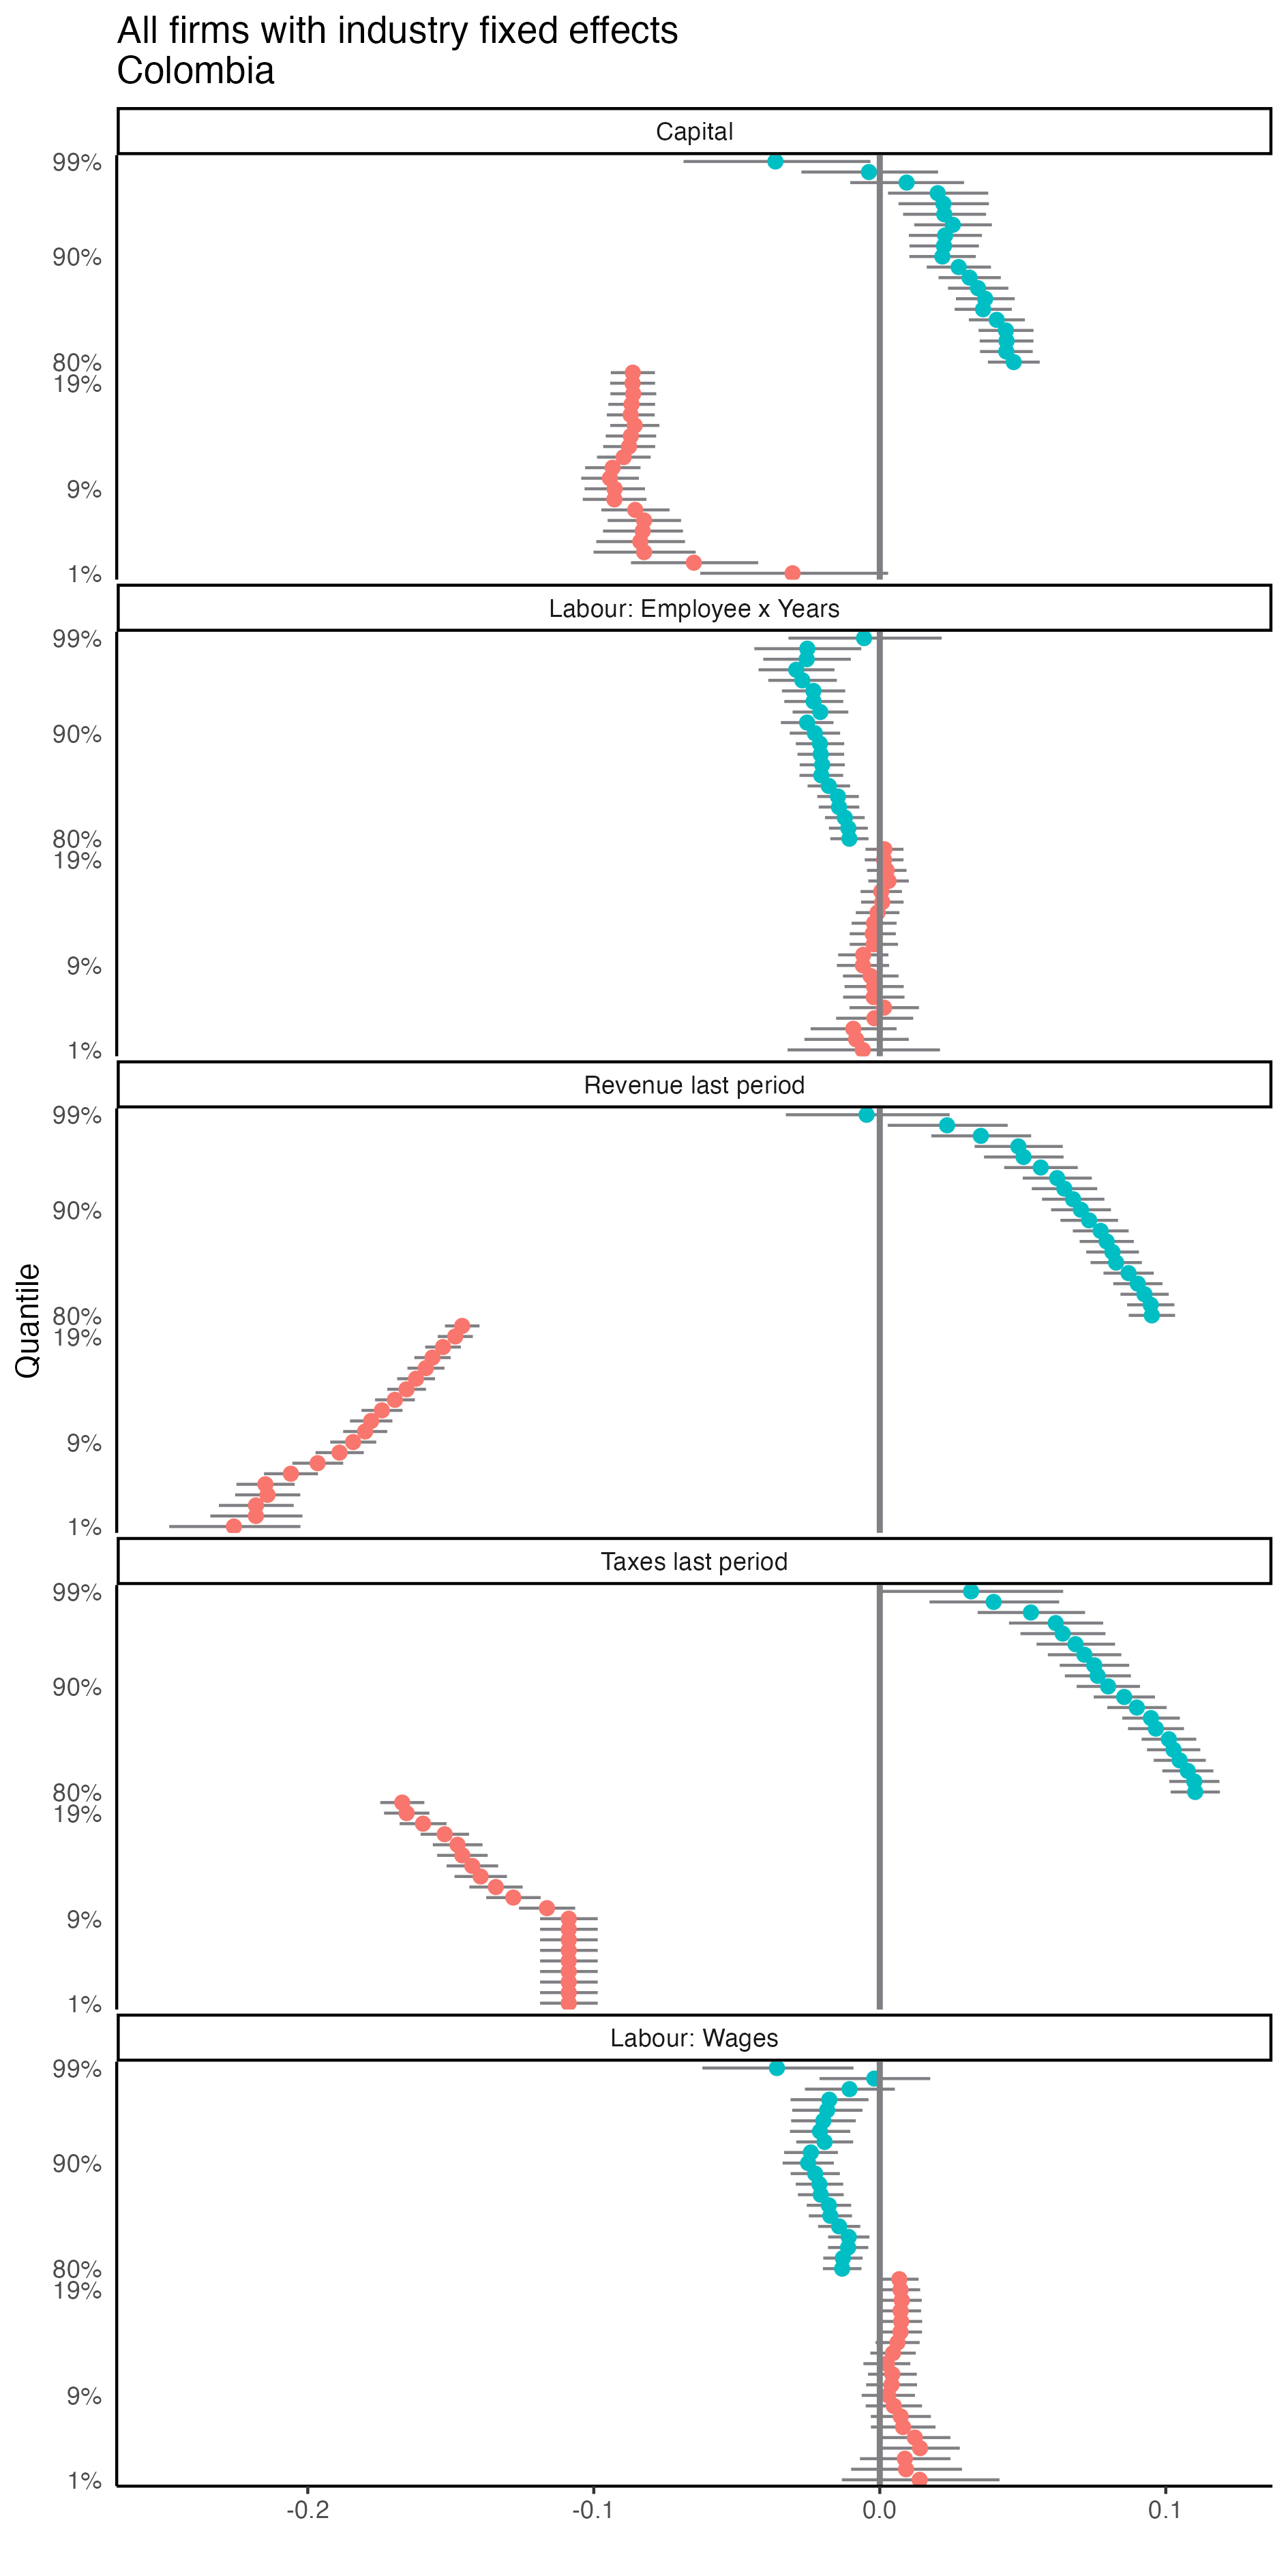
\includegraphics[width=\textwidth,height=1\textheight]{../Results/Figures/Colombia/beta_diff_all_fe.png}

}

\end{figure}

\begin{figure}

{\centering 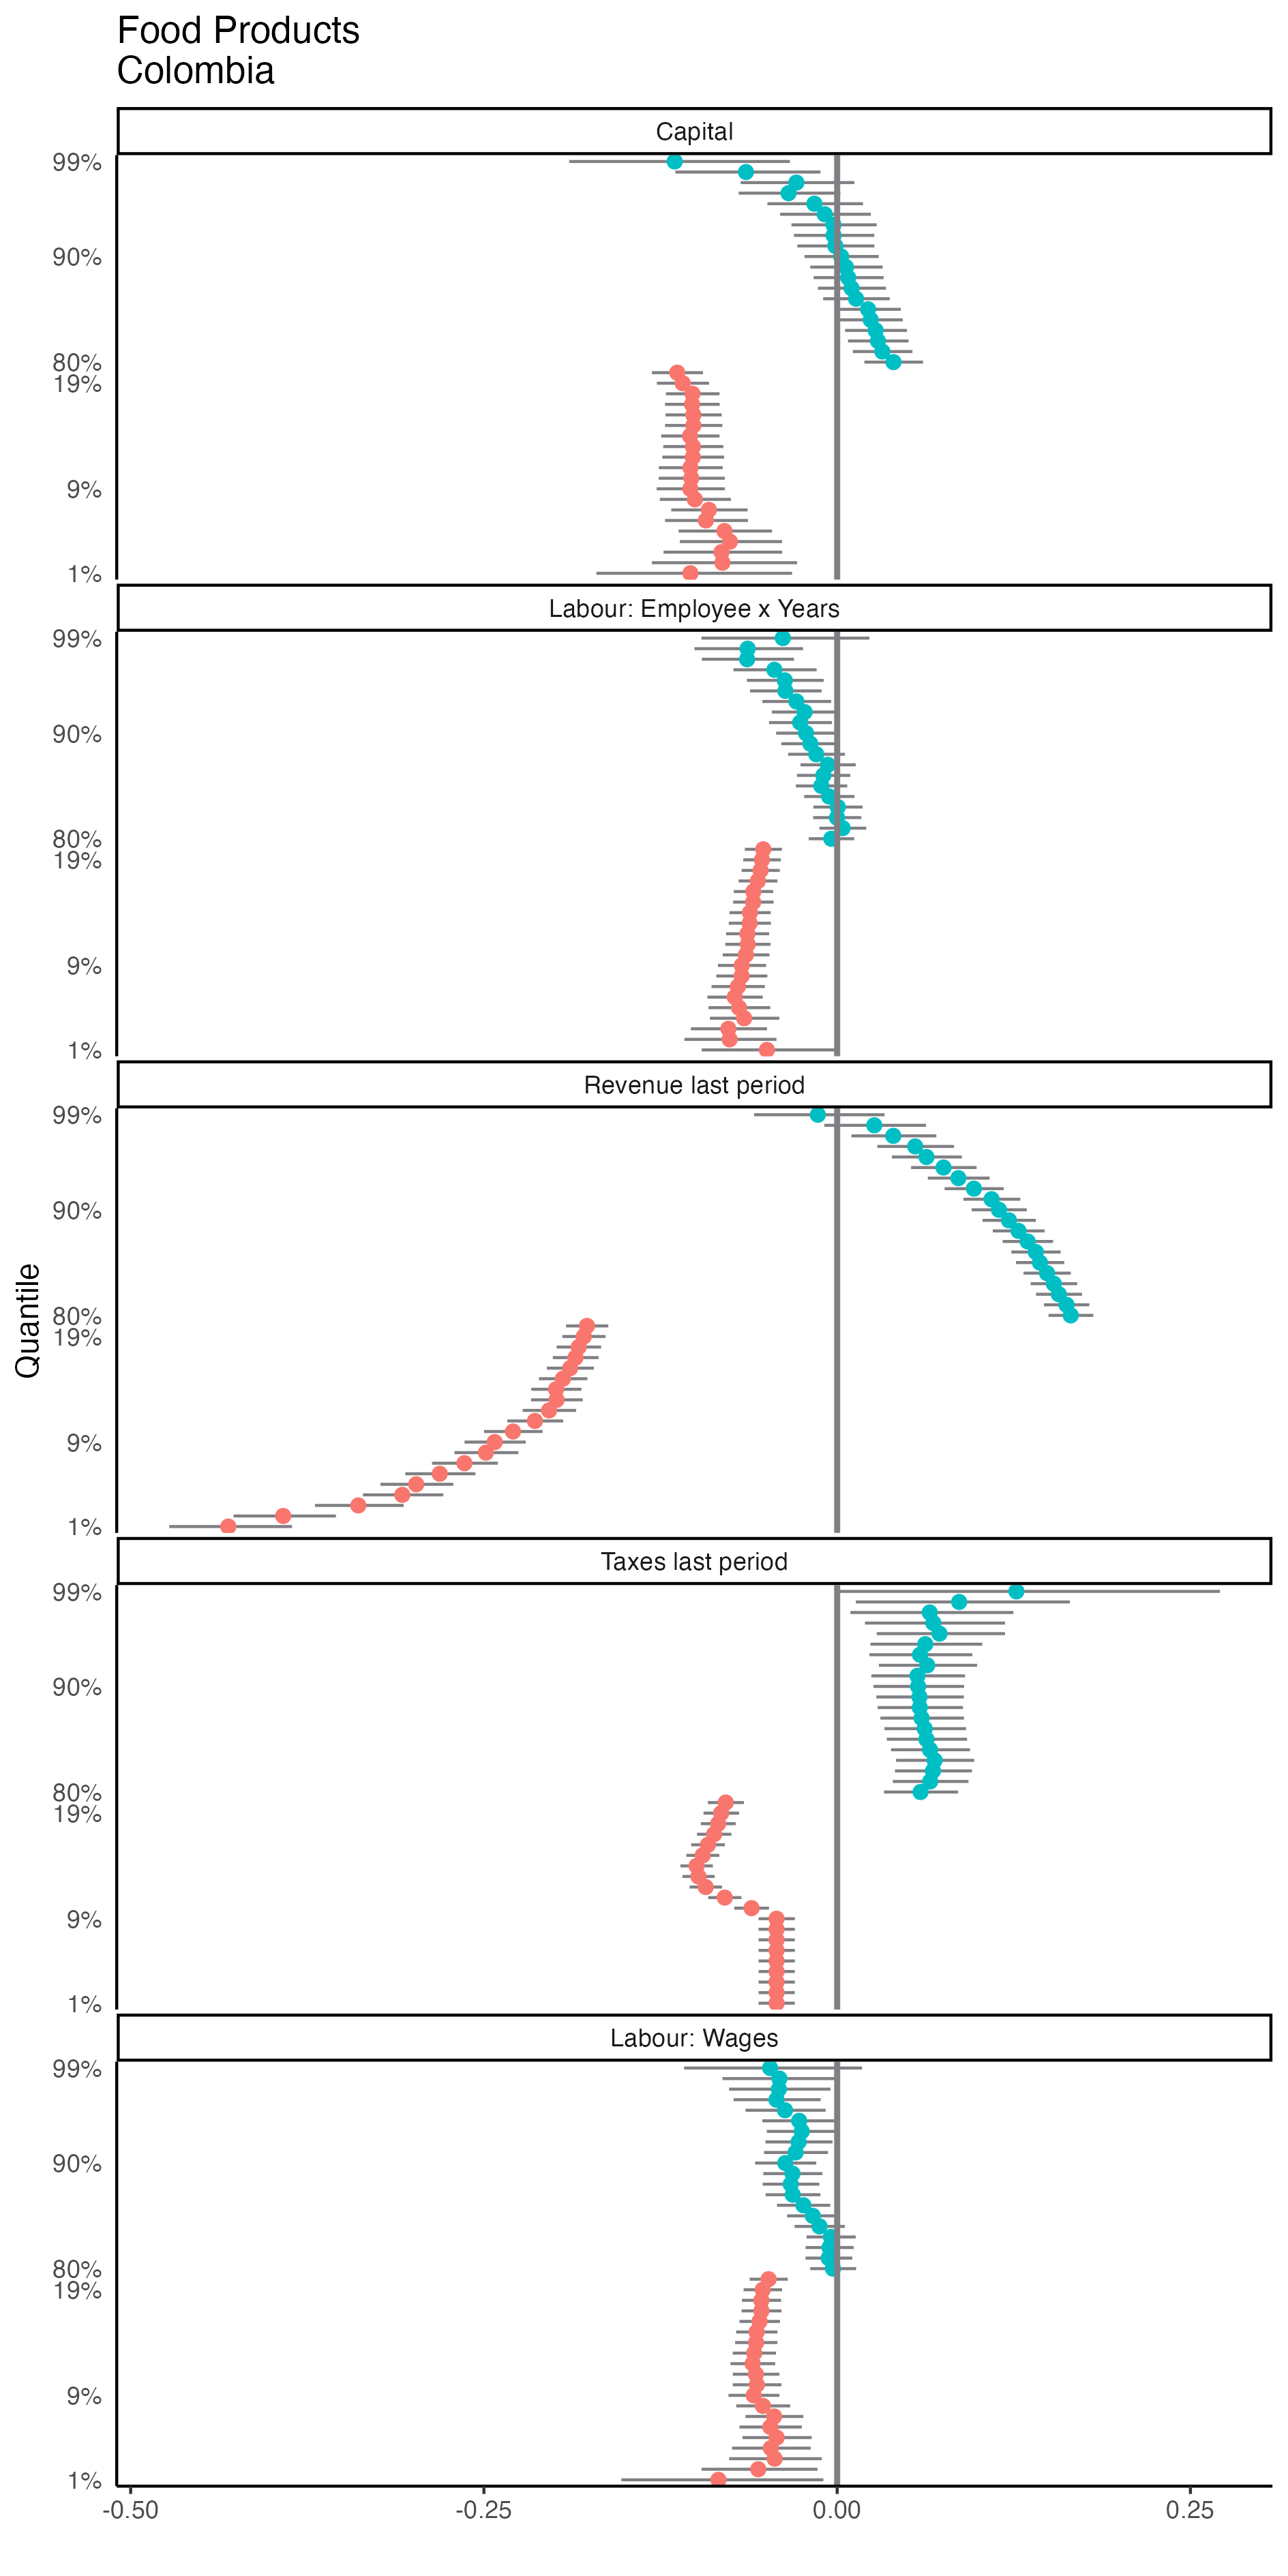
\includegraphics[width=\textwidth,height=1\textheight]{../Results/Figures/Colombia/311_by_size_diff.png}

}

\end{figure}

\begin{figure}

{\centering 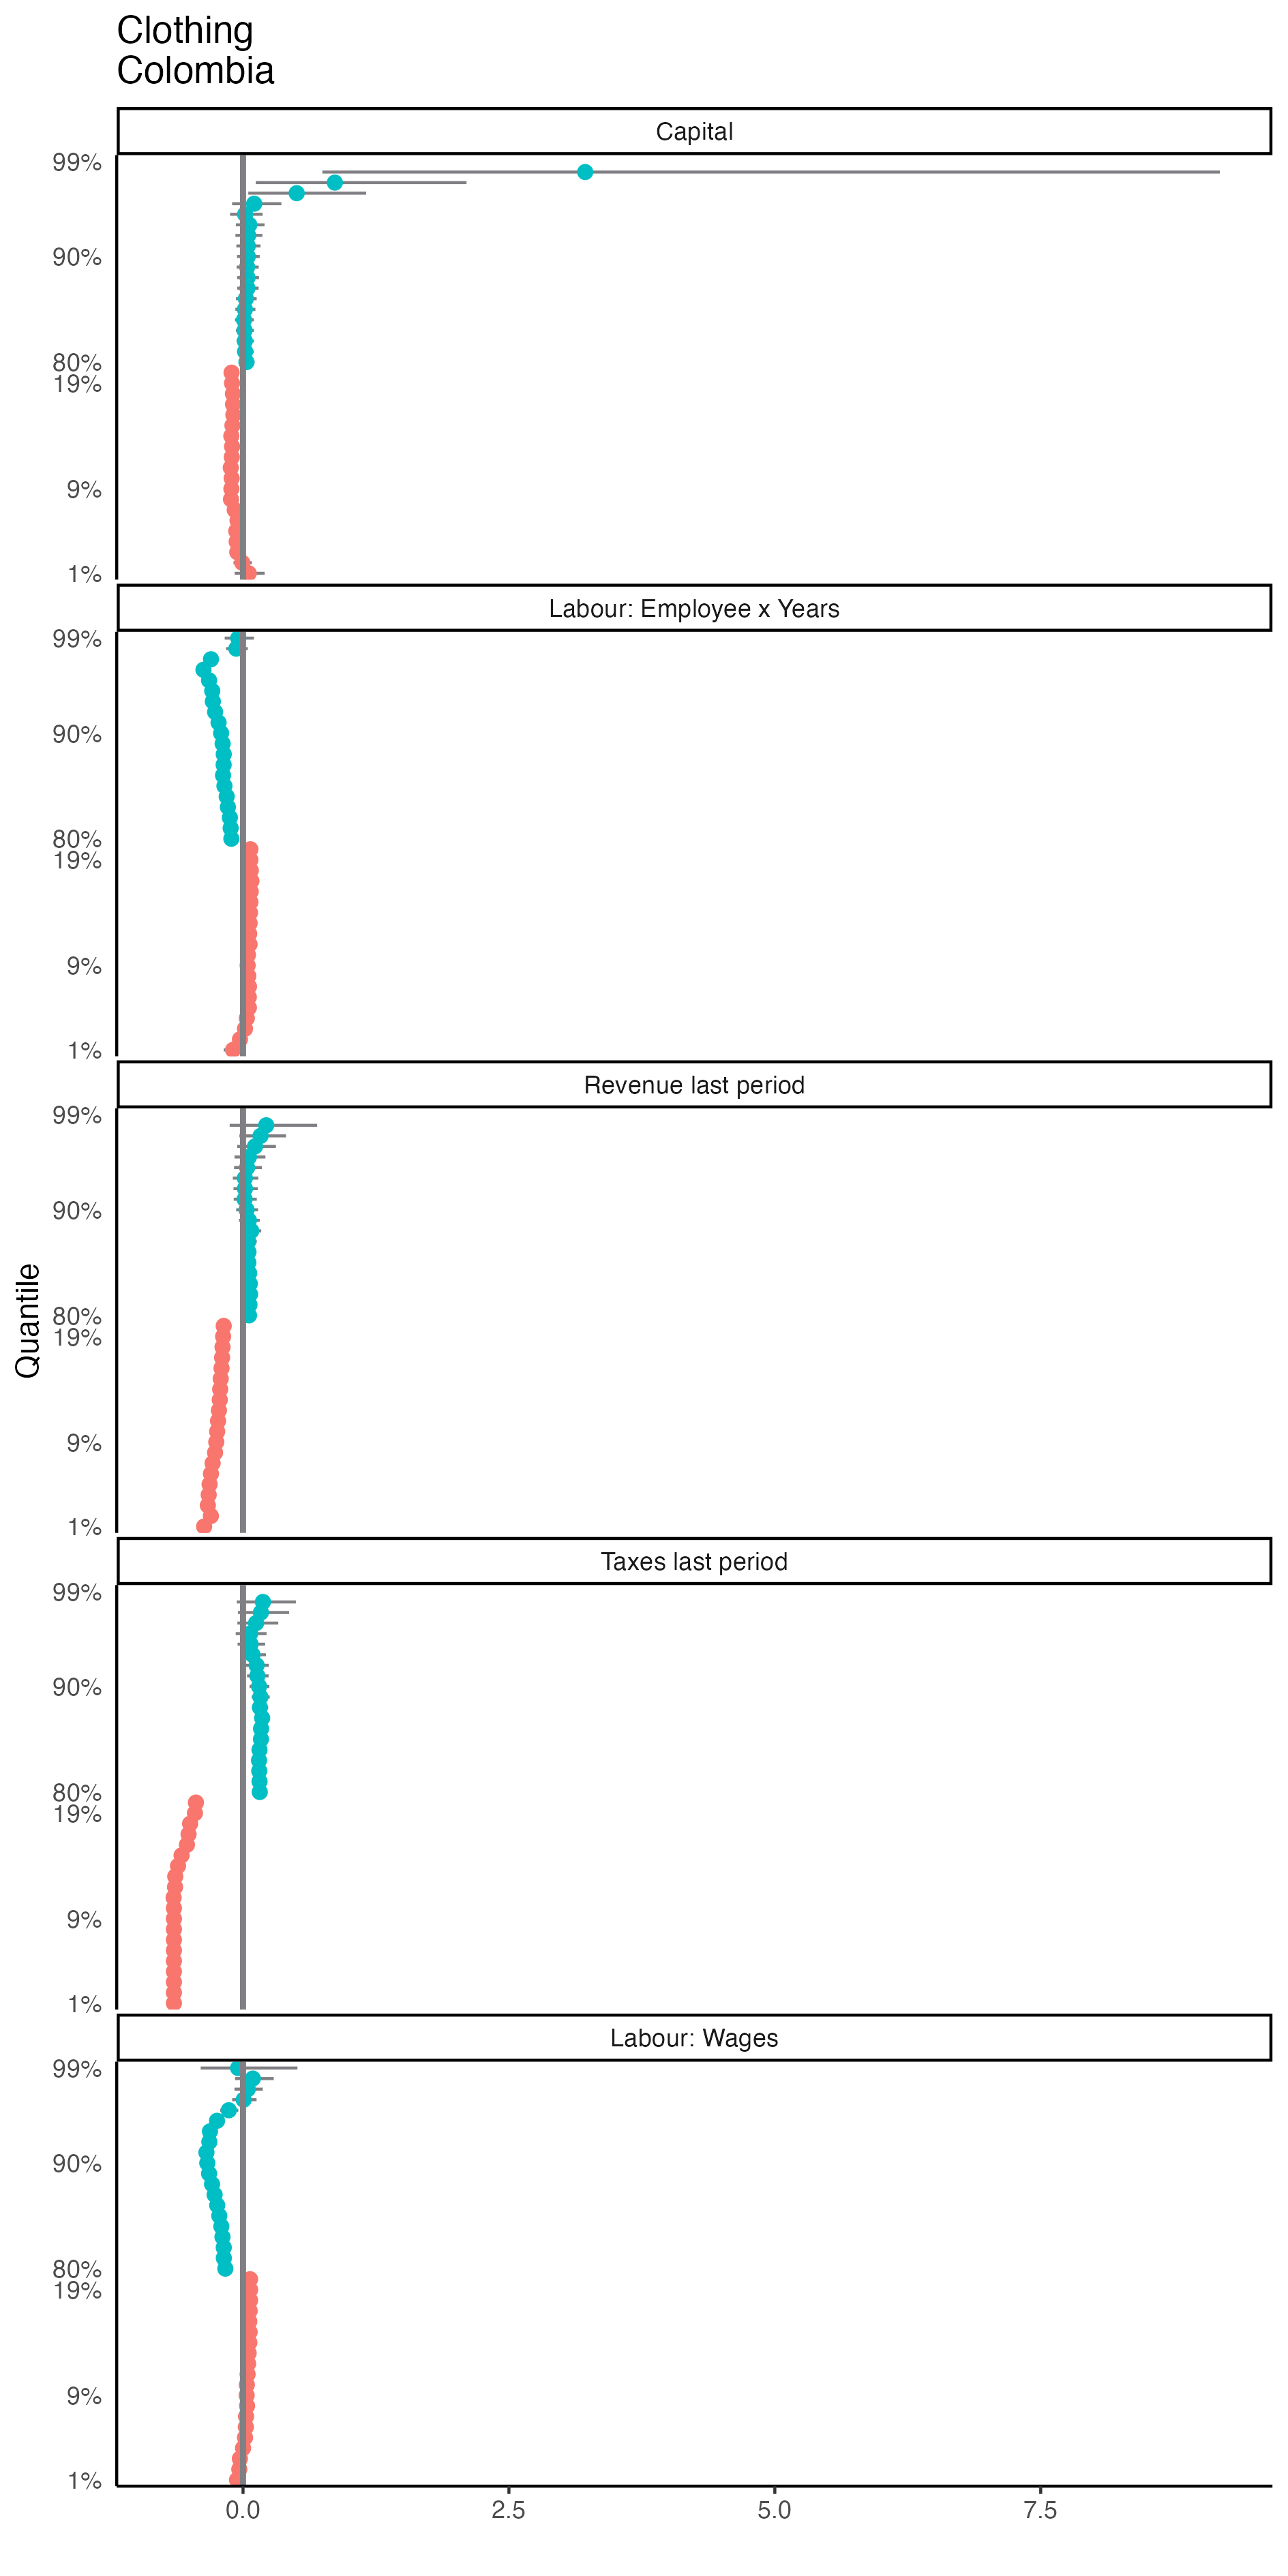
\includegraphics[width=\textwidth,height=1\textheight]{../Results/Figures/Colombia/322_by_size_diff.png}

}

\end{figure}

\begin{figure}

{\centering 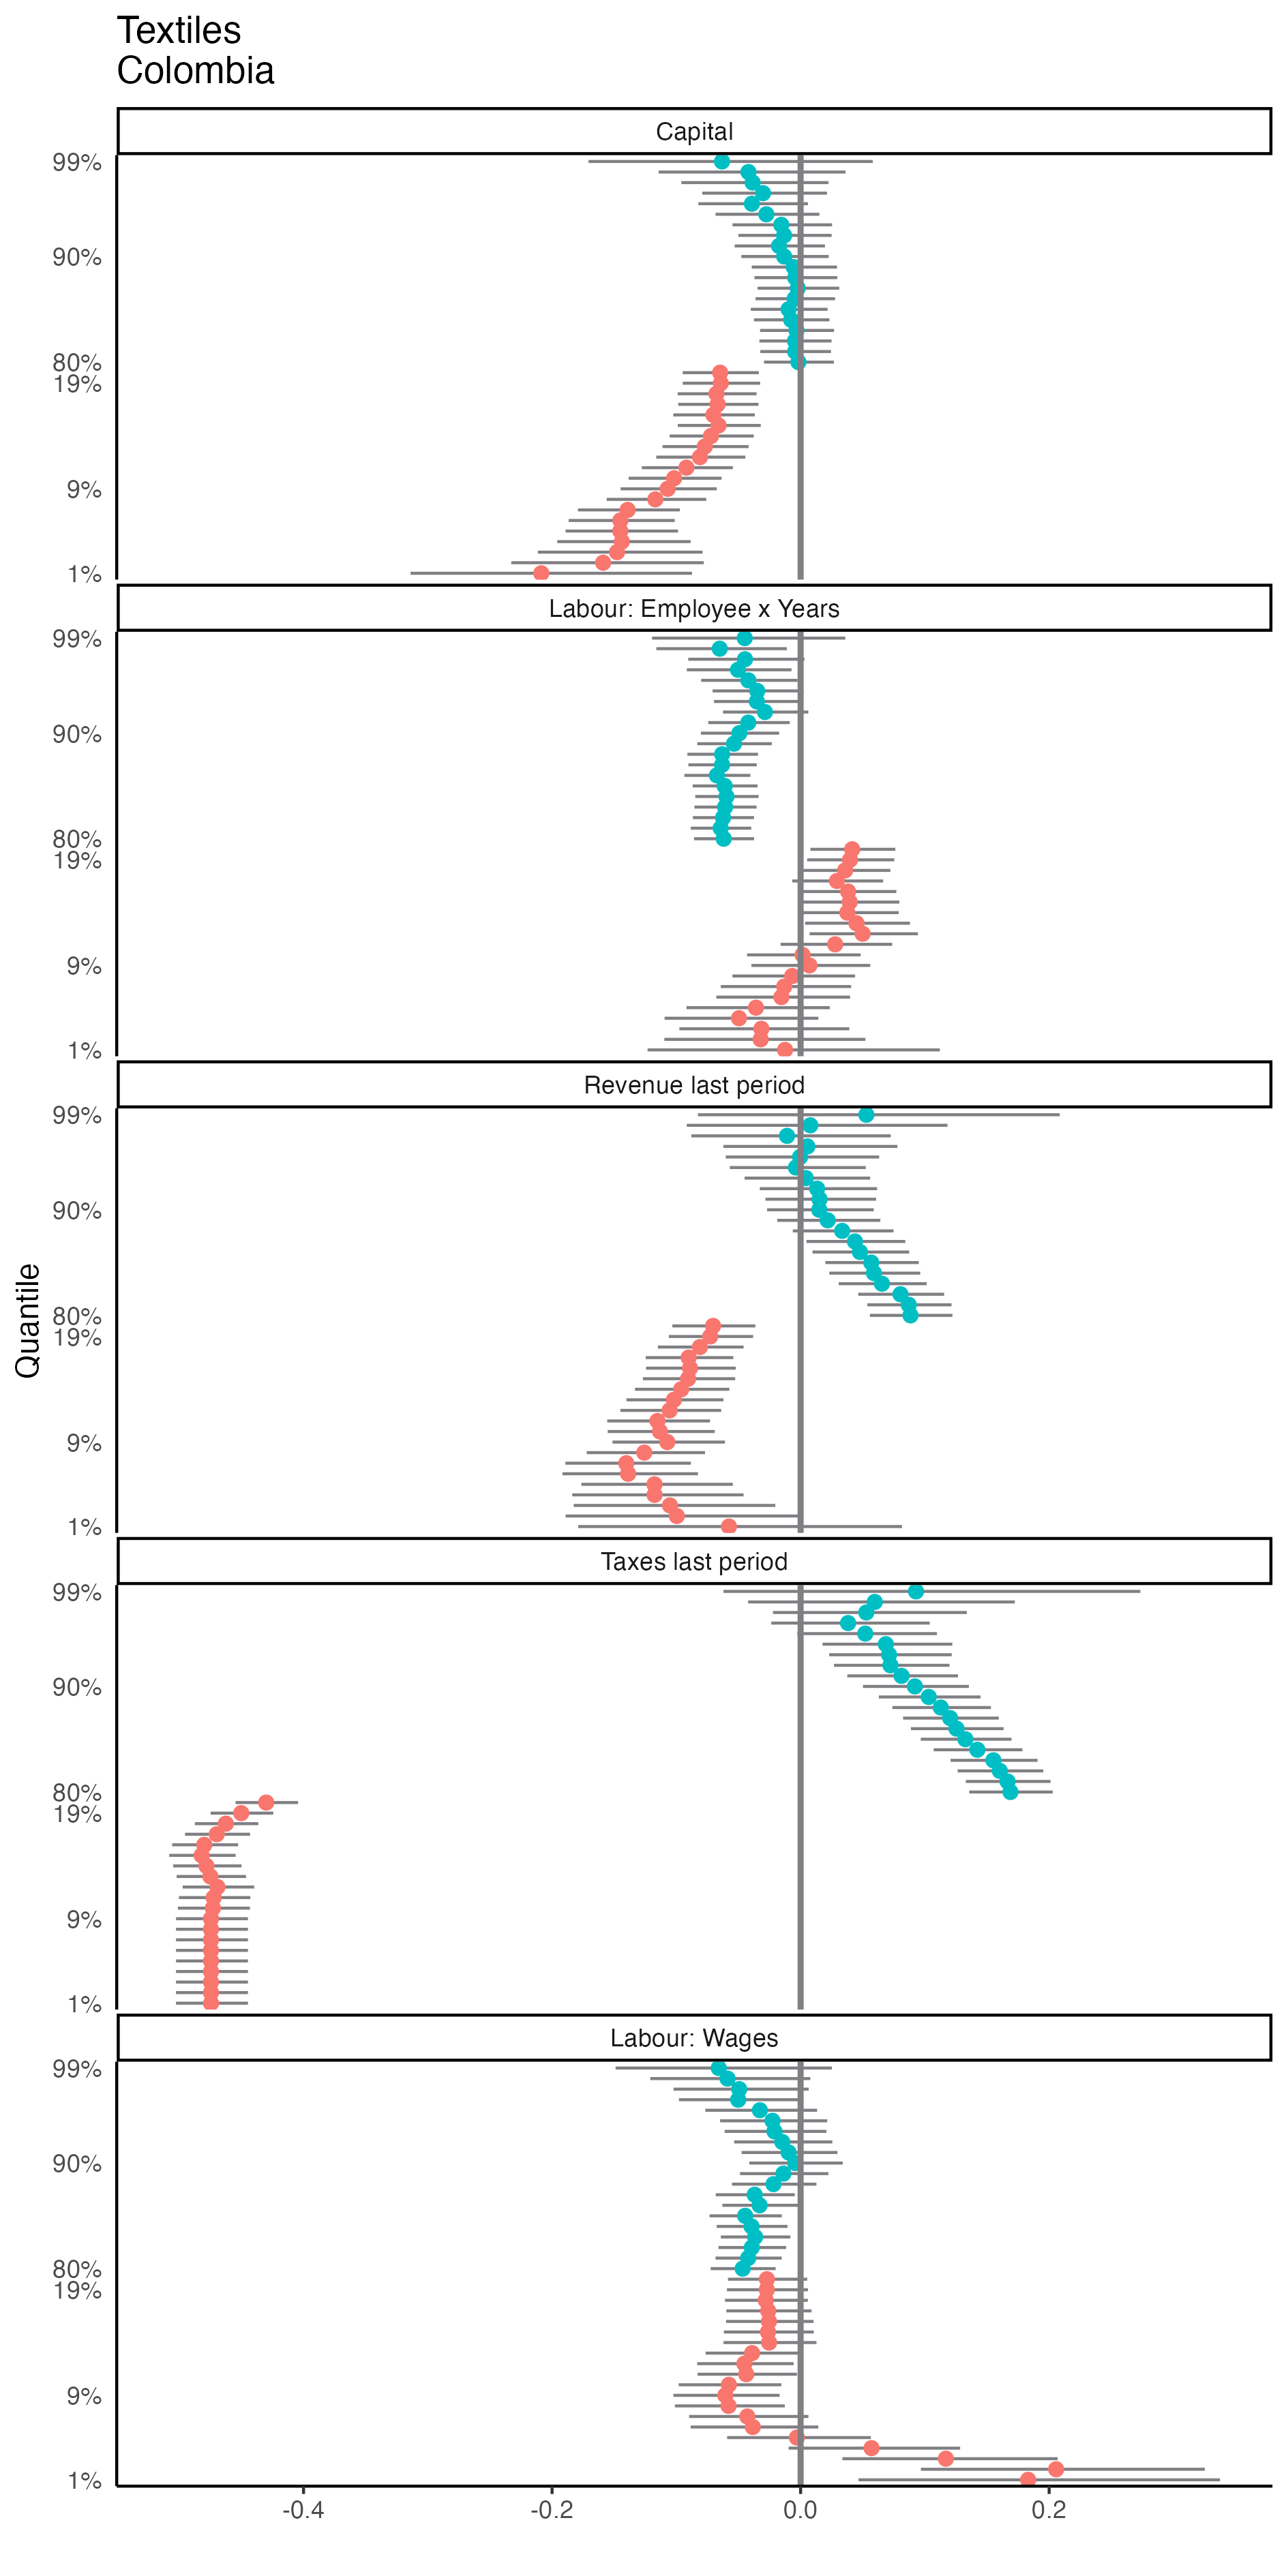
\includegraphics[width=\textwidth,height=1\textheight]{../Results/Figures/Colombia/321_by_size_diff.png}

}

\end{figure}

\begin{figure}

{\centering 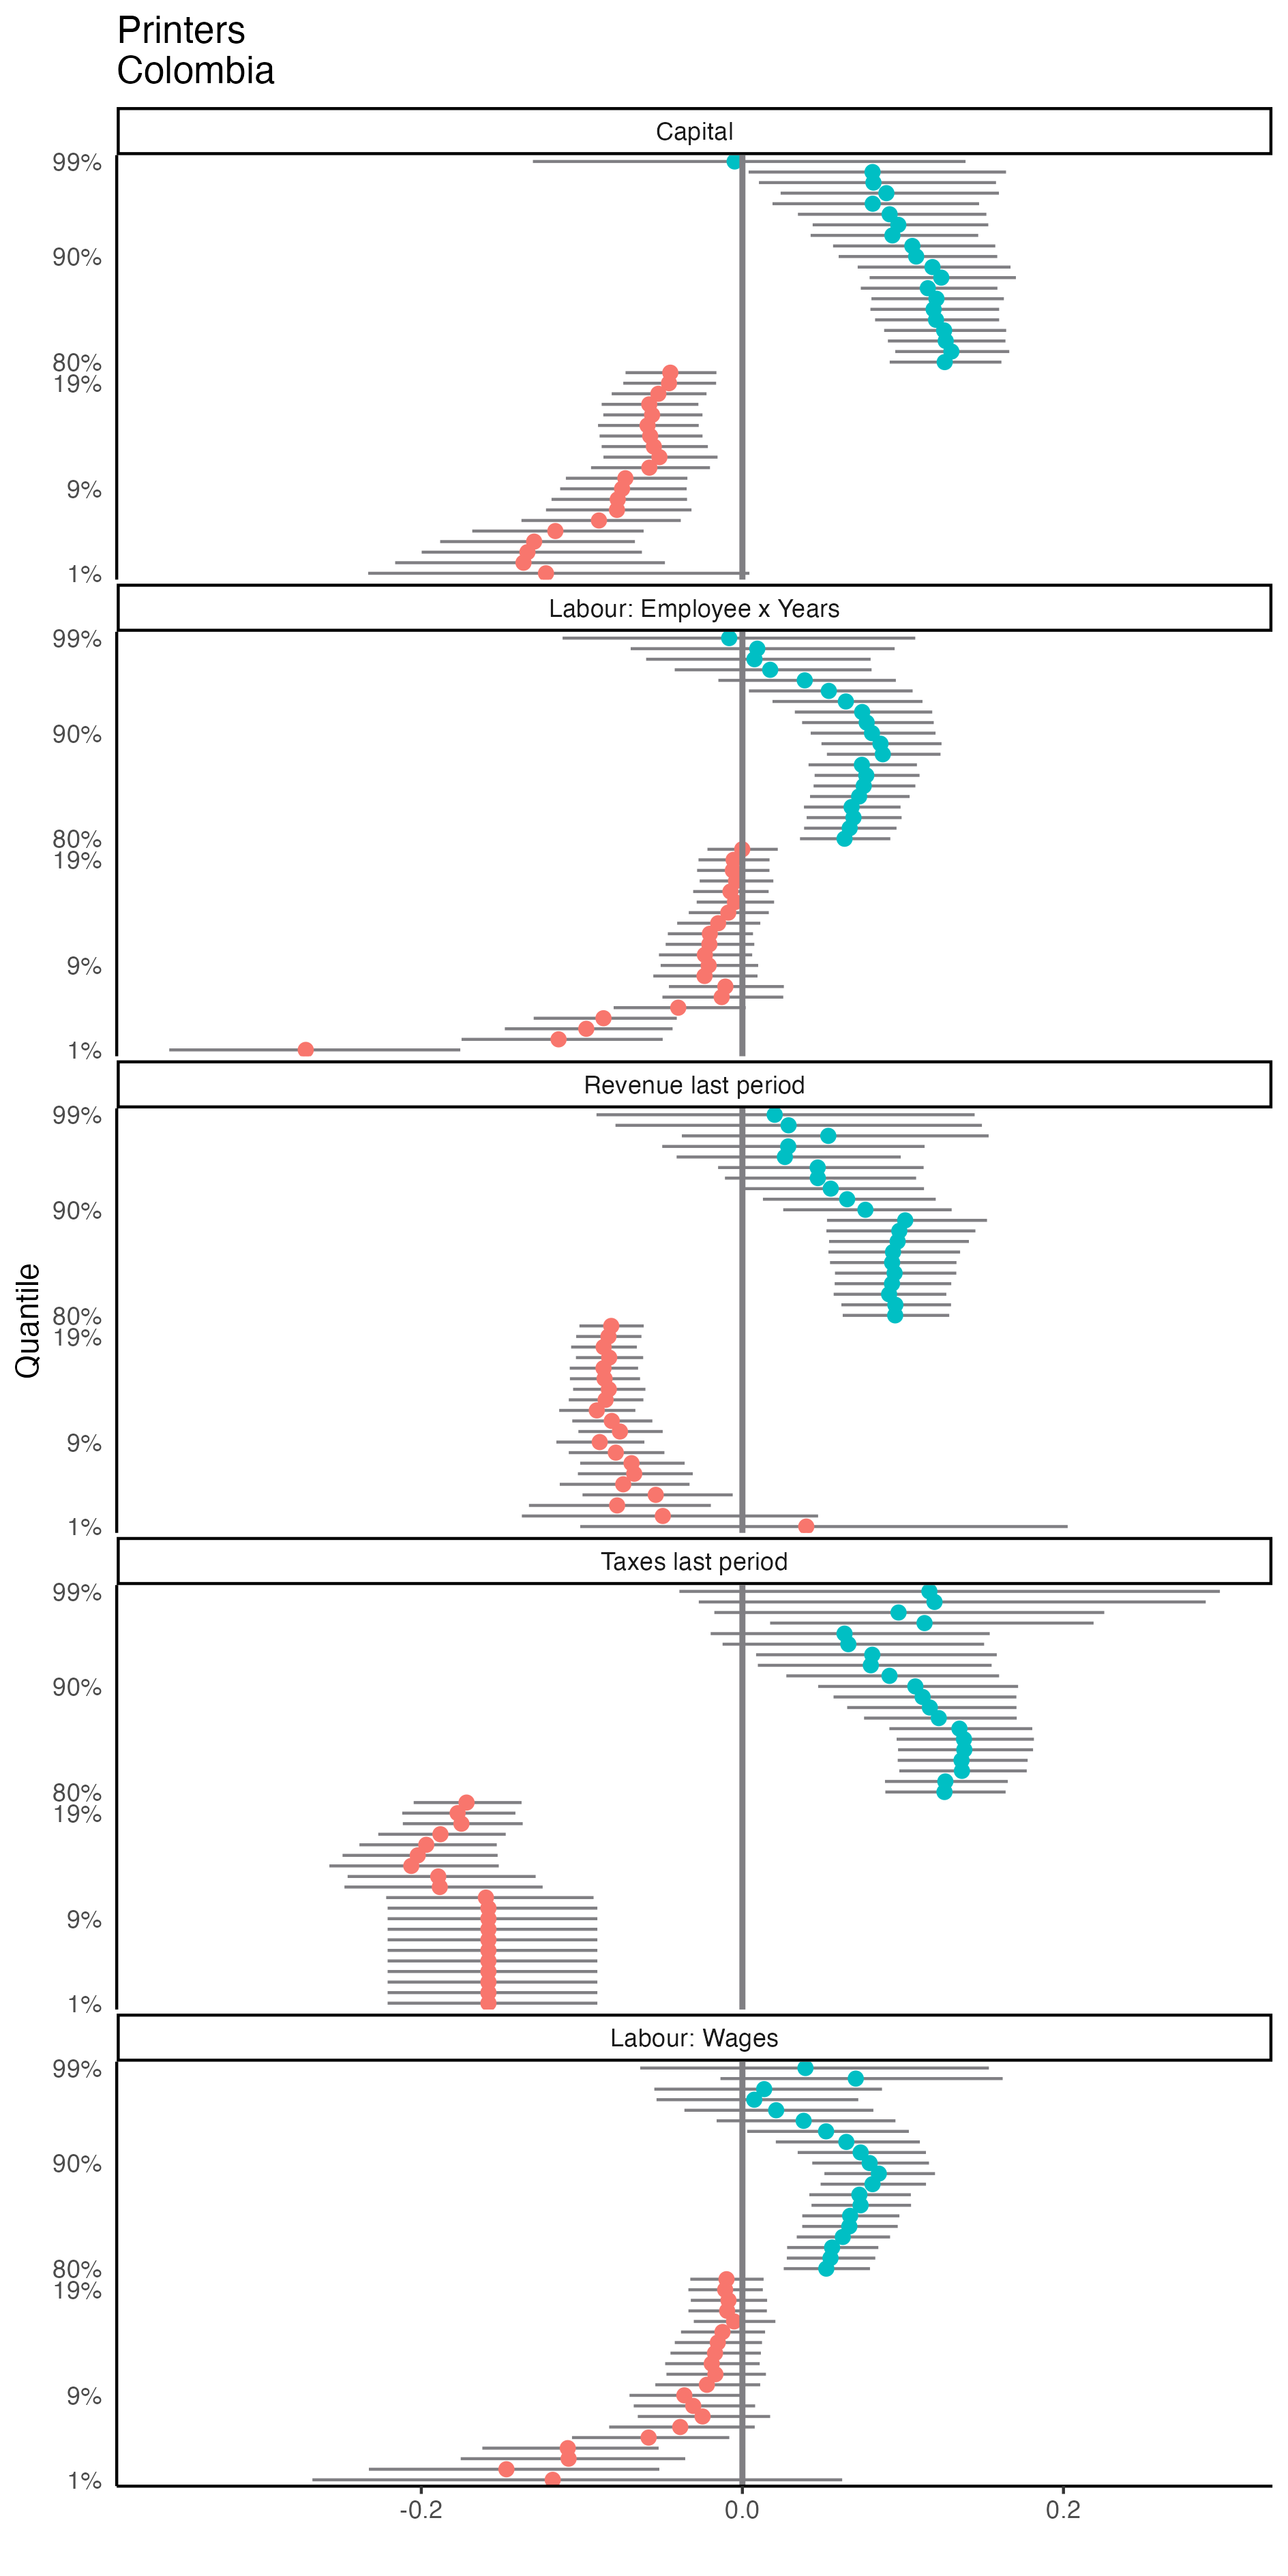
\includegraphics[width=\textwidth,height=1\textheight]{../Results/Figures/Colombia/342_by_size_diff.png}

}

\end{figure}

\begin{figure}

{\centering 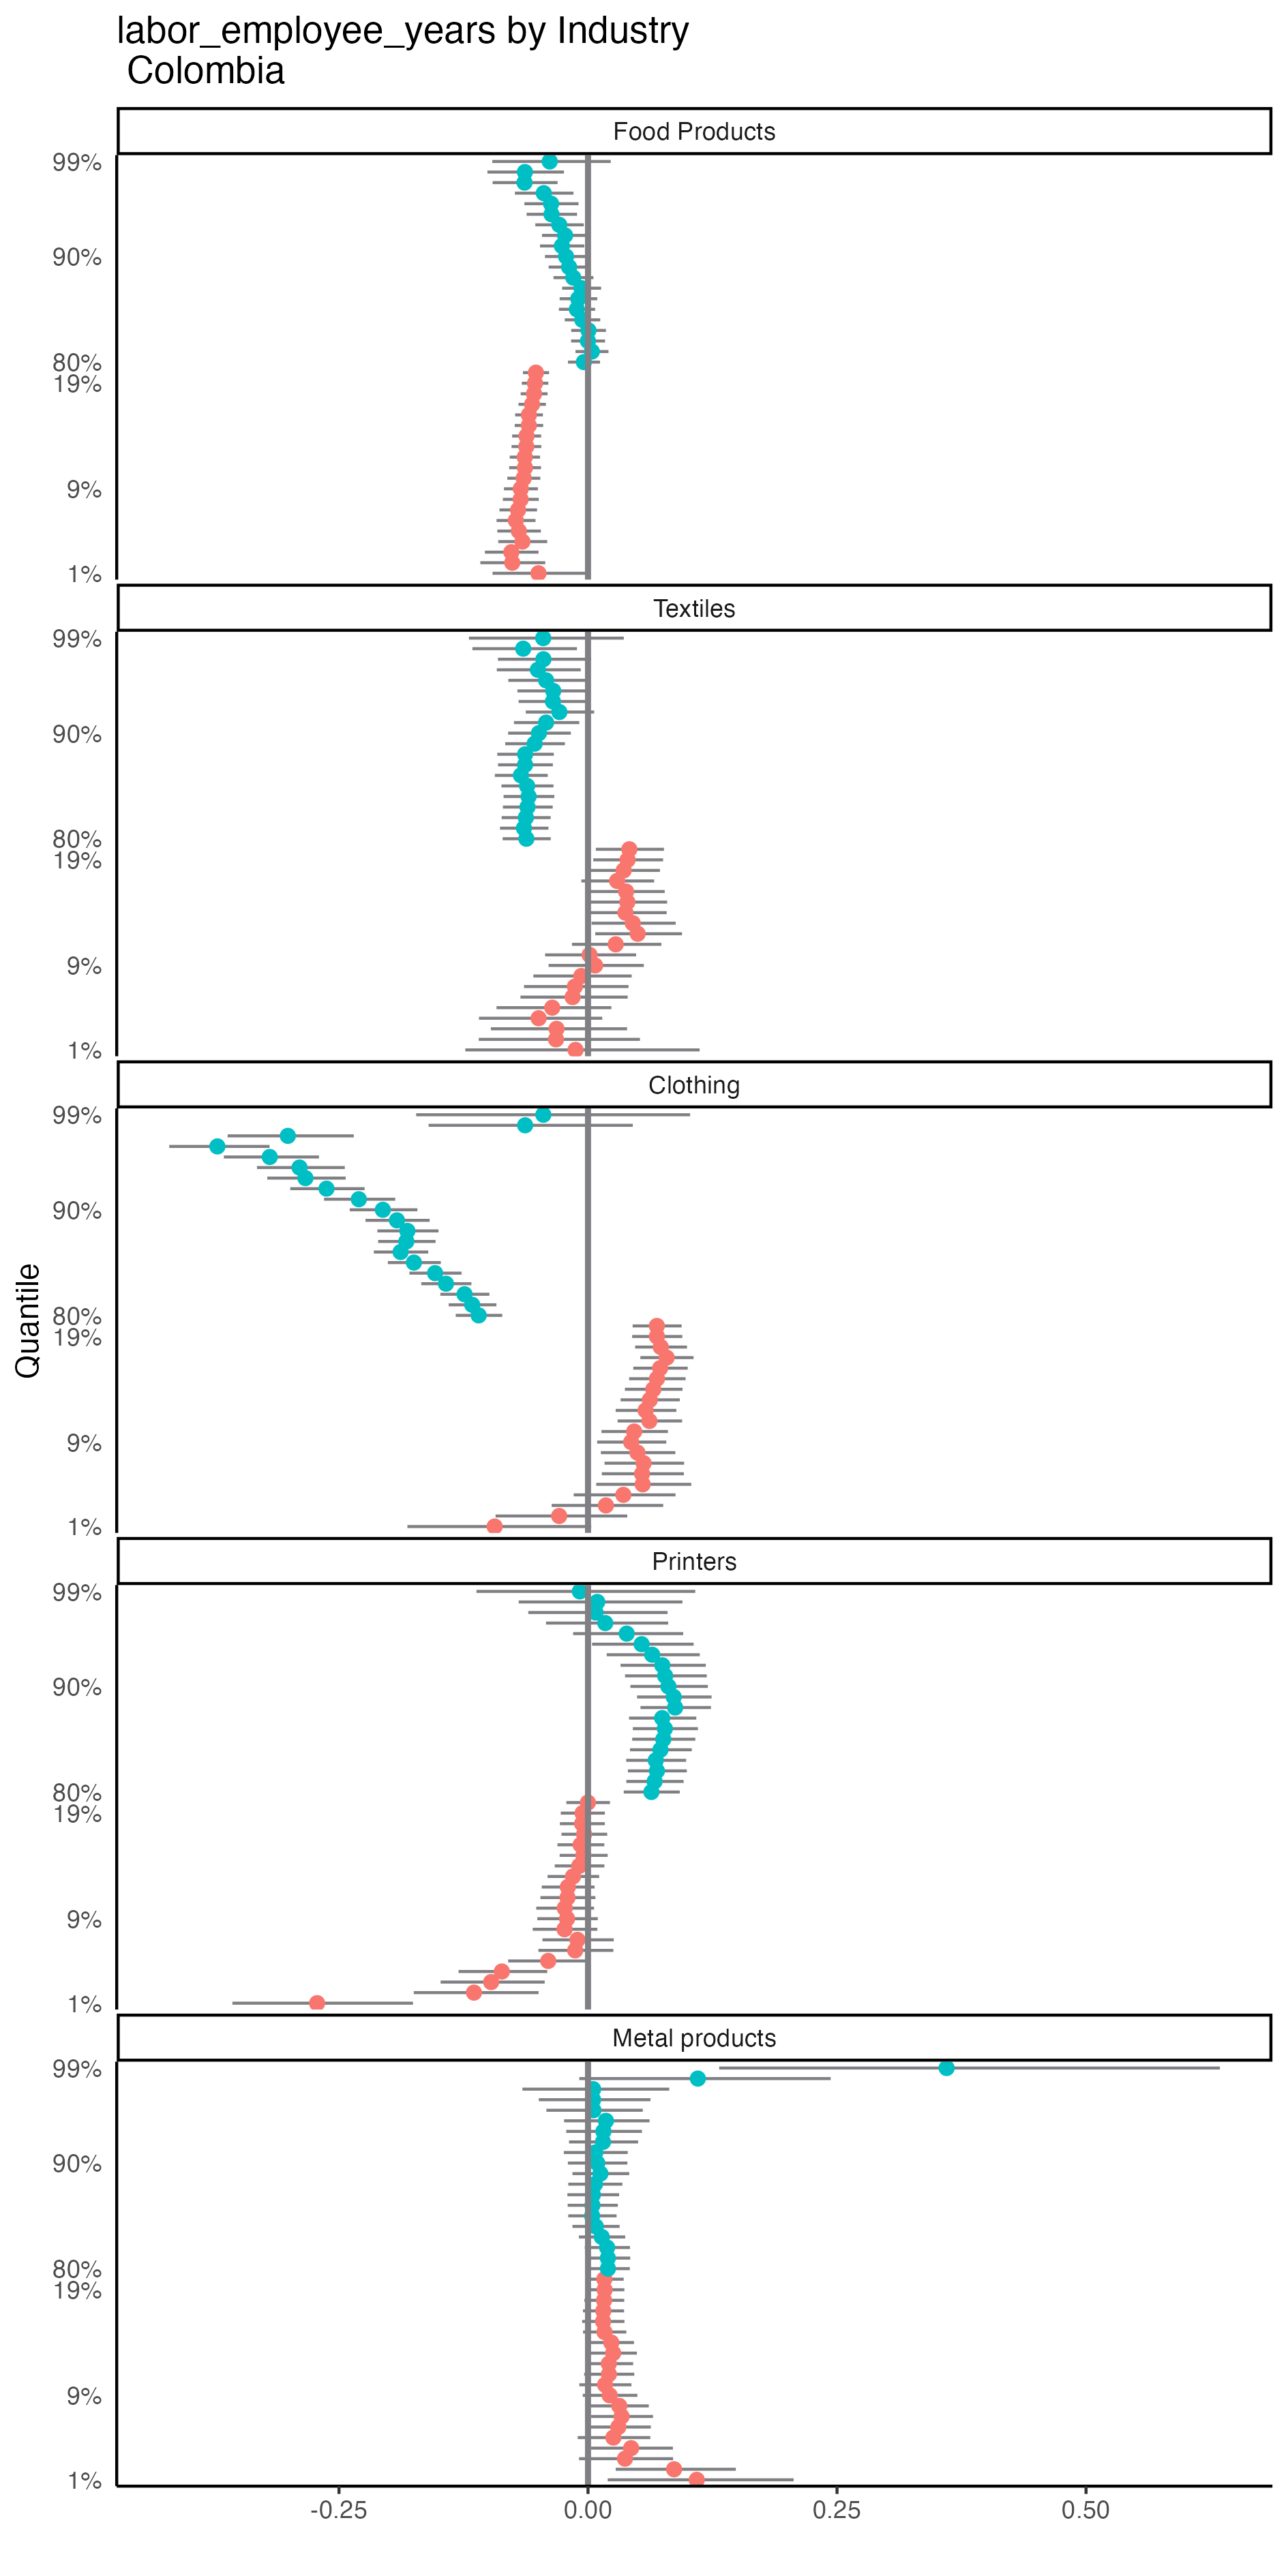
\includegraphics[width=\textwidth,height=1\textheight]{../Results/Figures/Colombia/labor_employee_years_by_inds_diff.png}

}

\end{figure}

\begin{figure}

{\centering 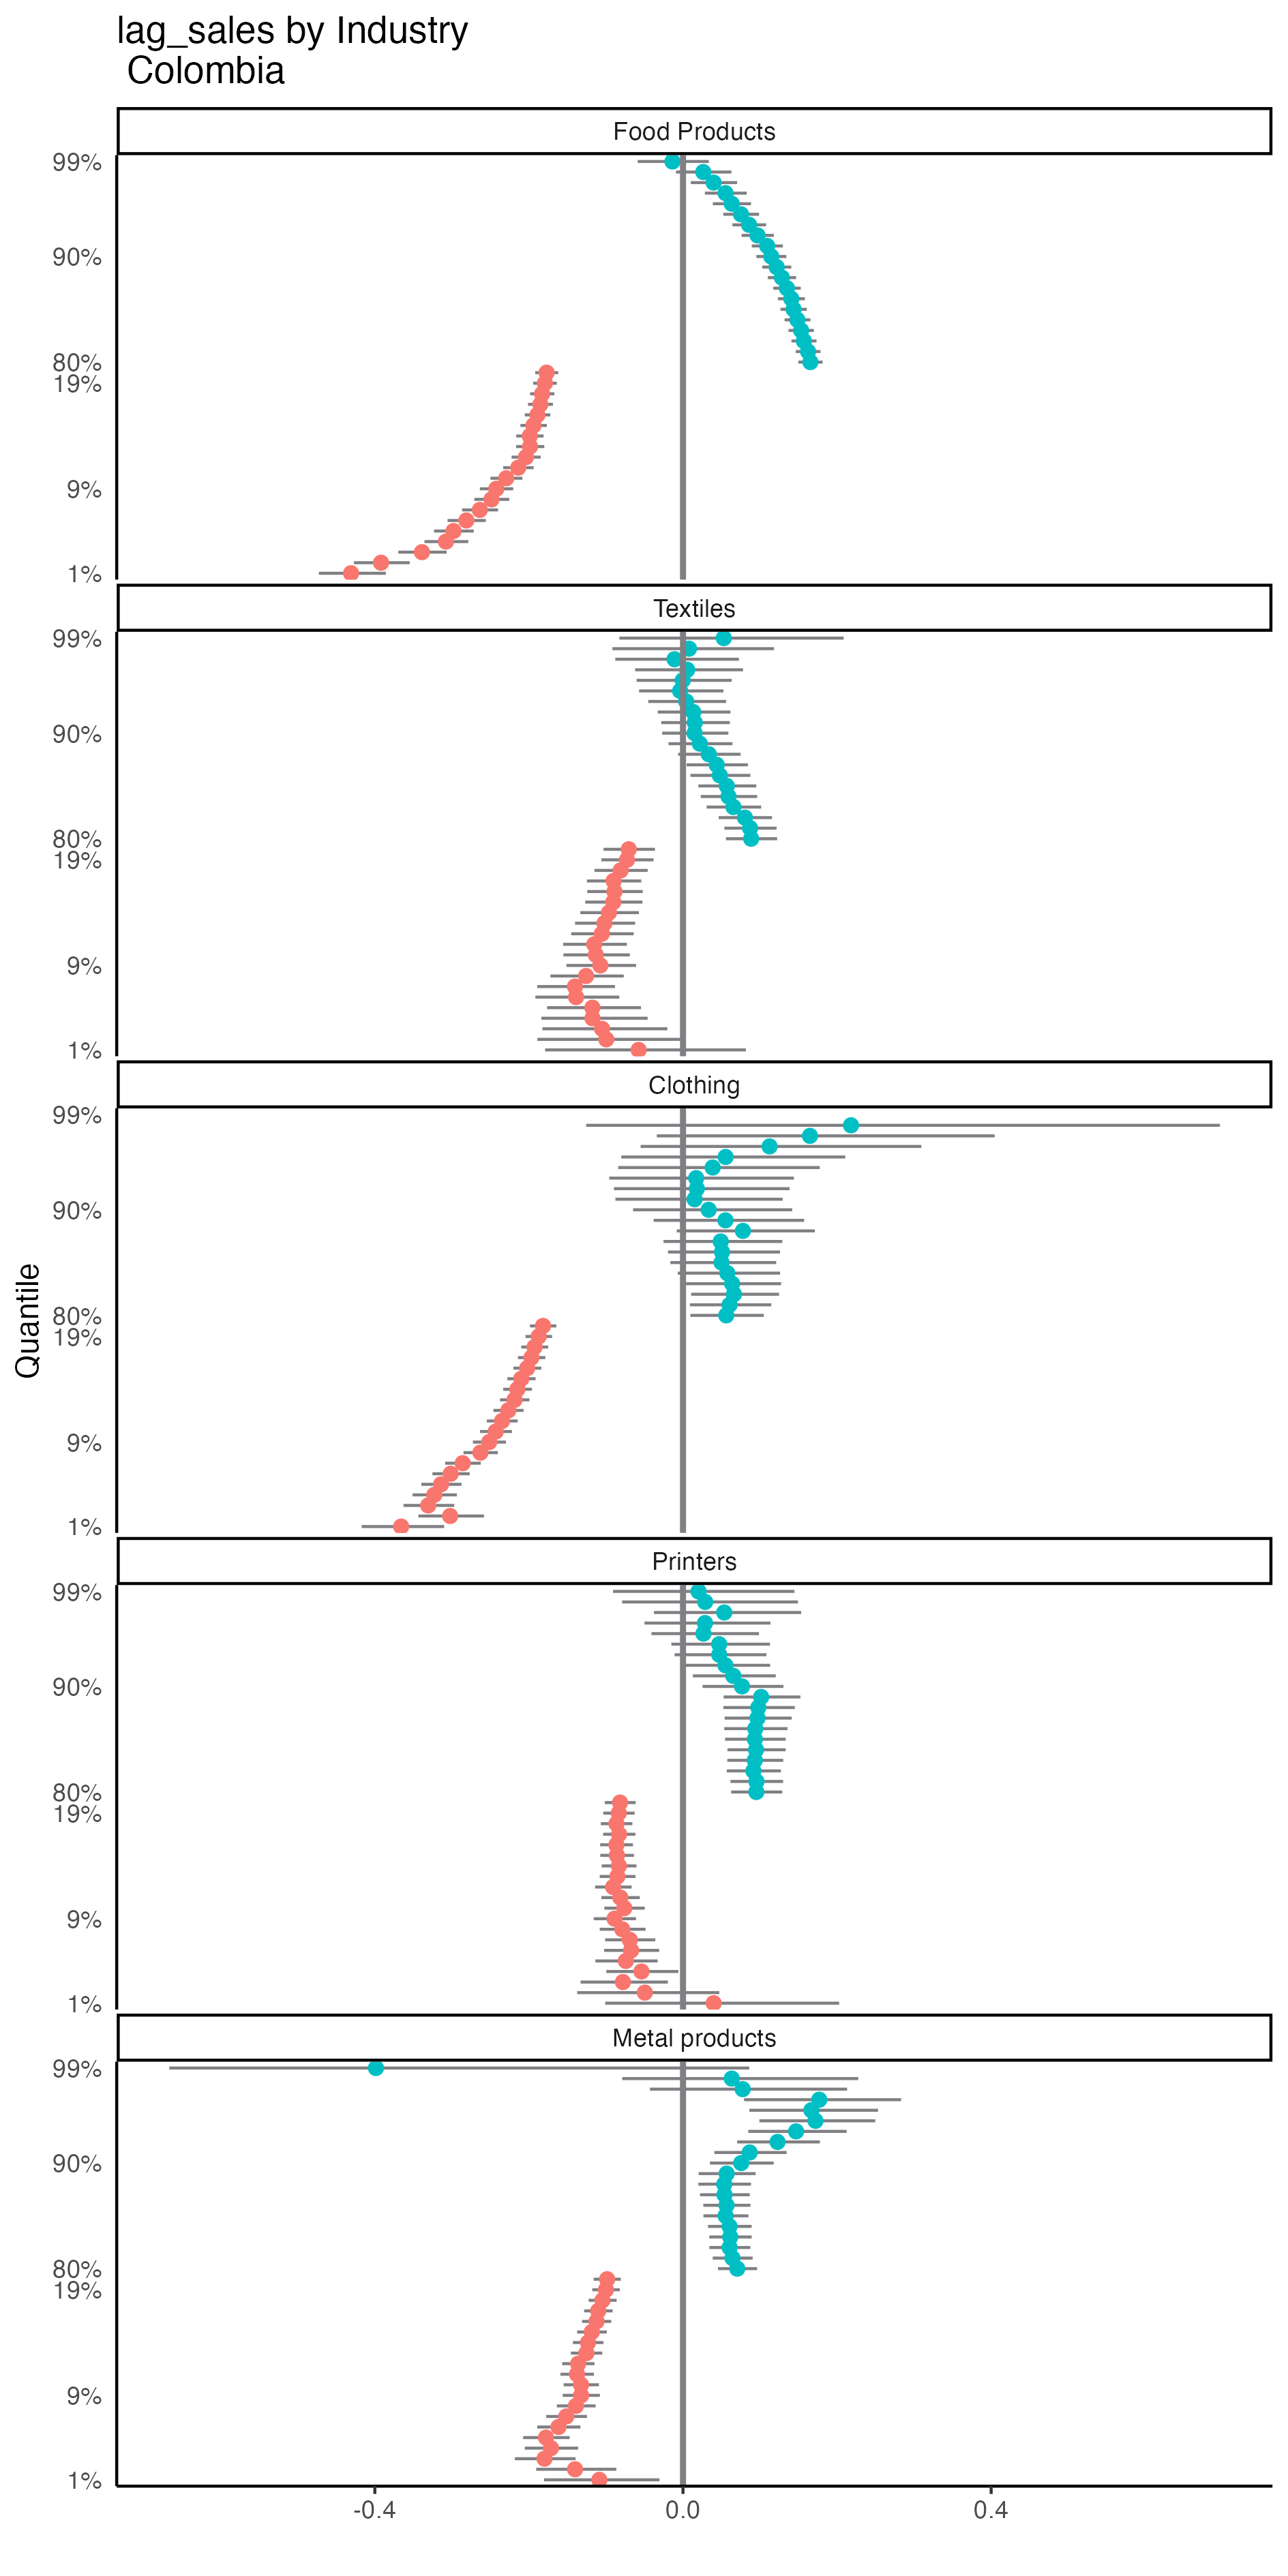
\includegraphics[width=\textwidth,height=1\textheight]{../Results/Figures/Colombia/lag_sales_by_inds_diff.png}

}

\end{figure}

\begin{figure}

{\centering 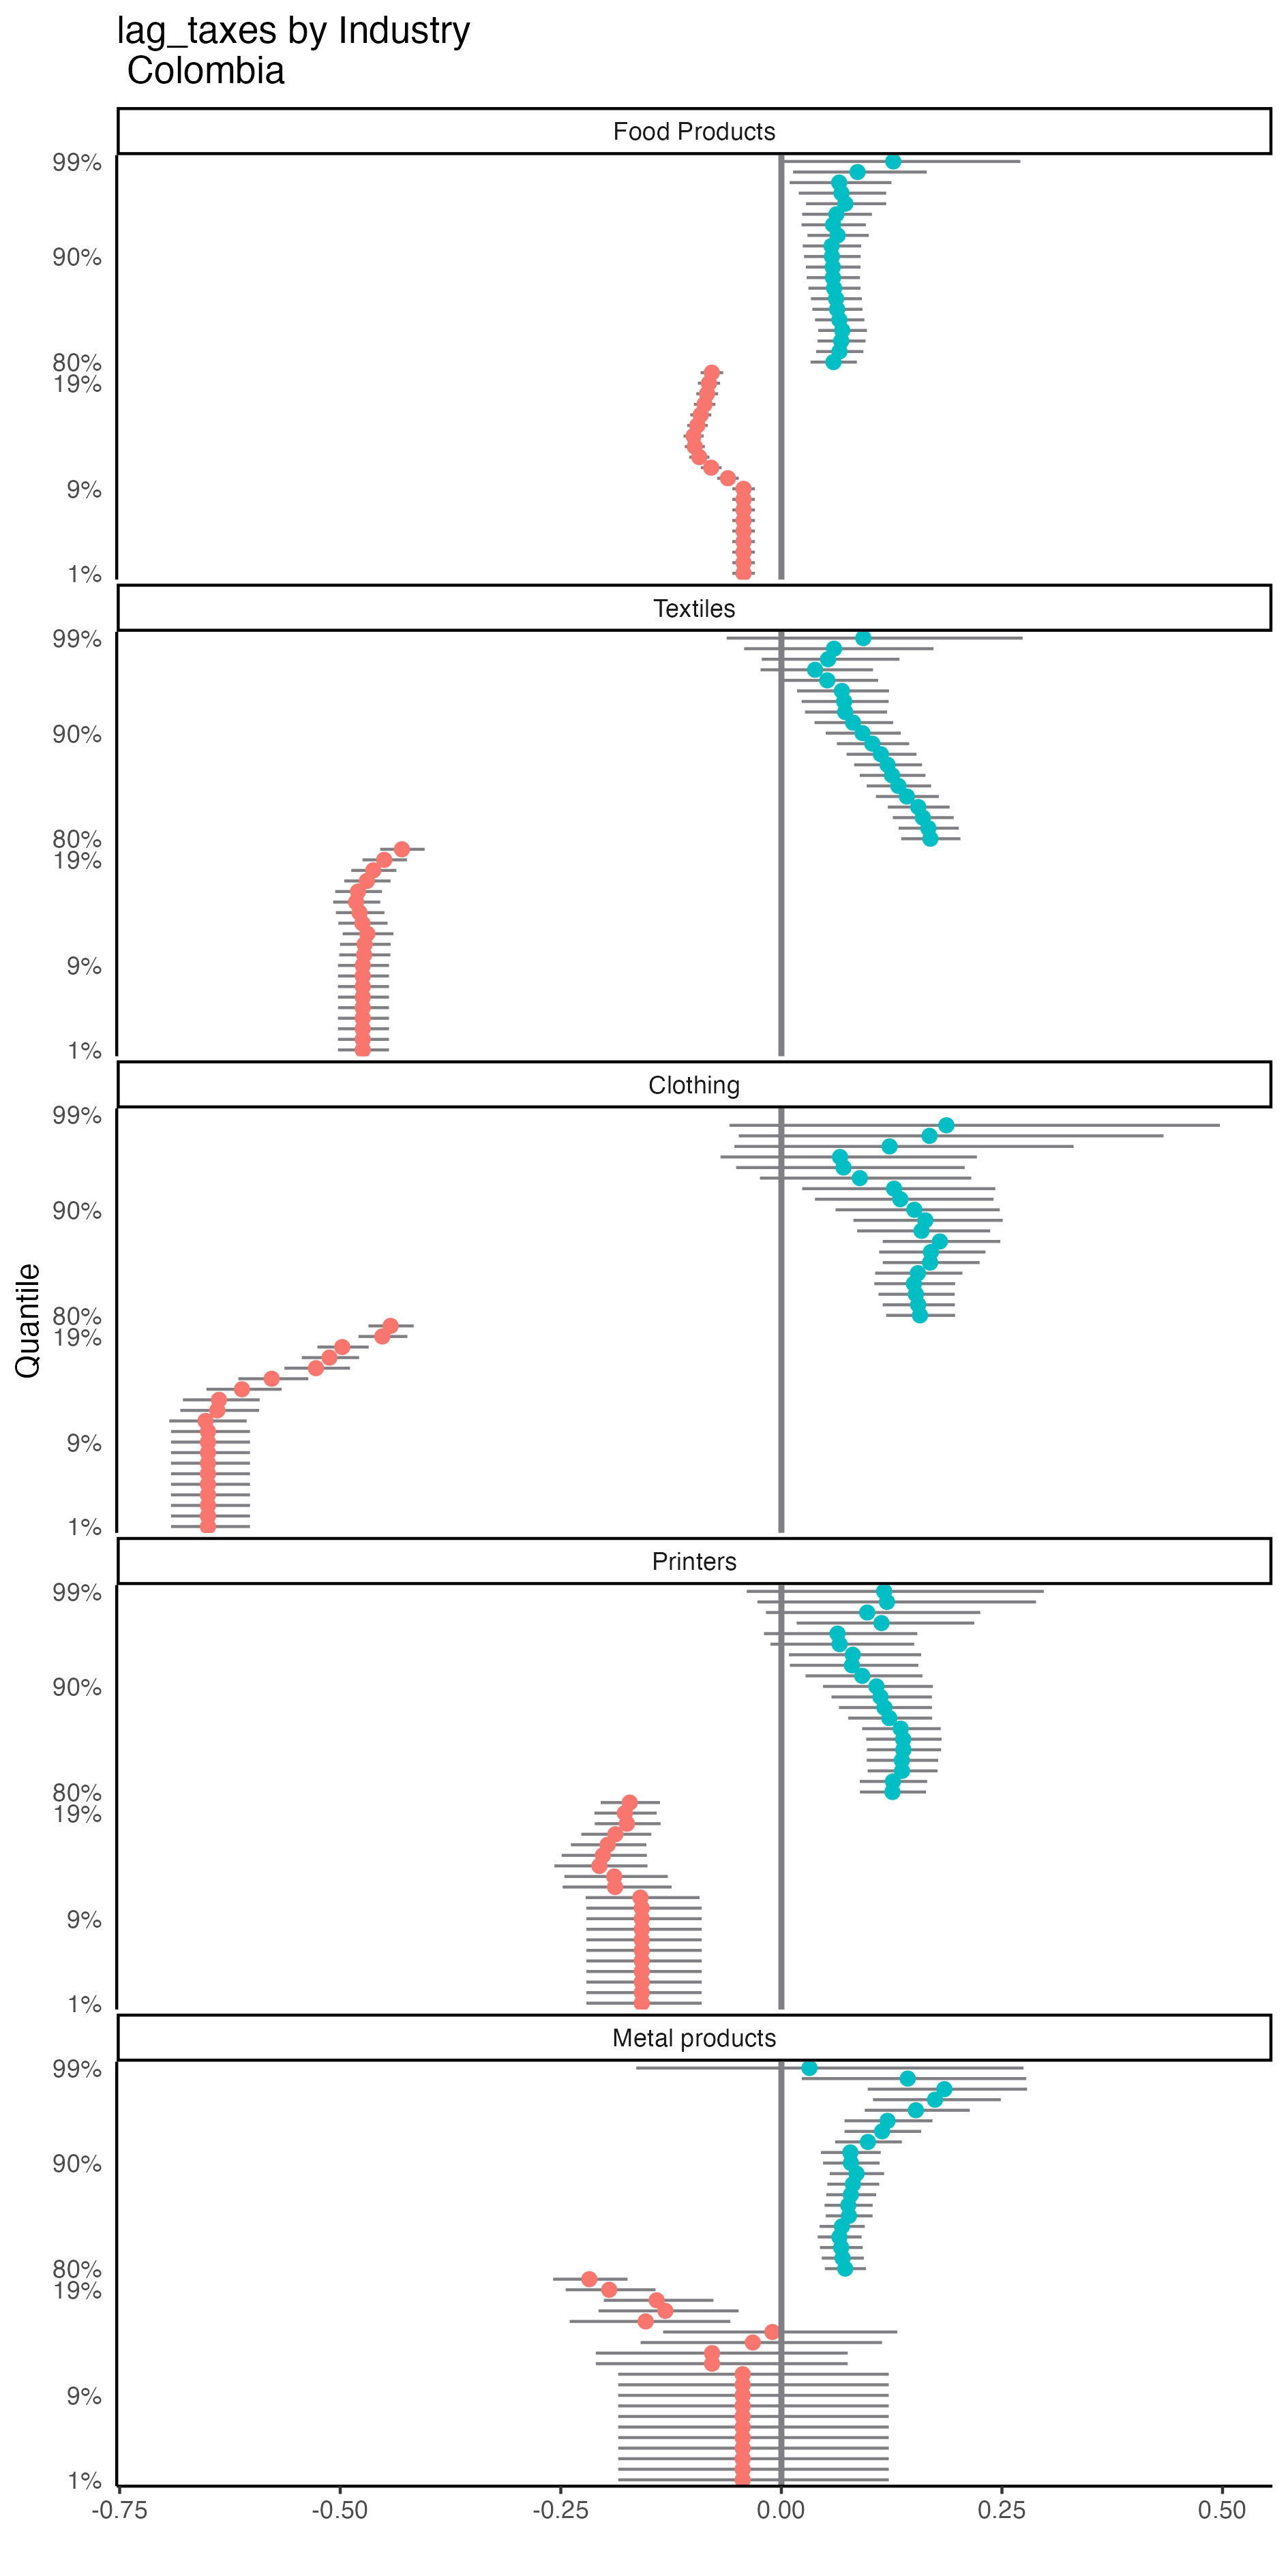
\includegraphics[width=\textwidth,height=1\textheight]{../Results/Figures/Colombia/lag_taxes_by_inds_diff.png}

}

\end{figure}

\begin{figure}

{\centering 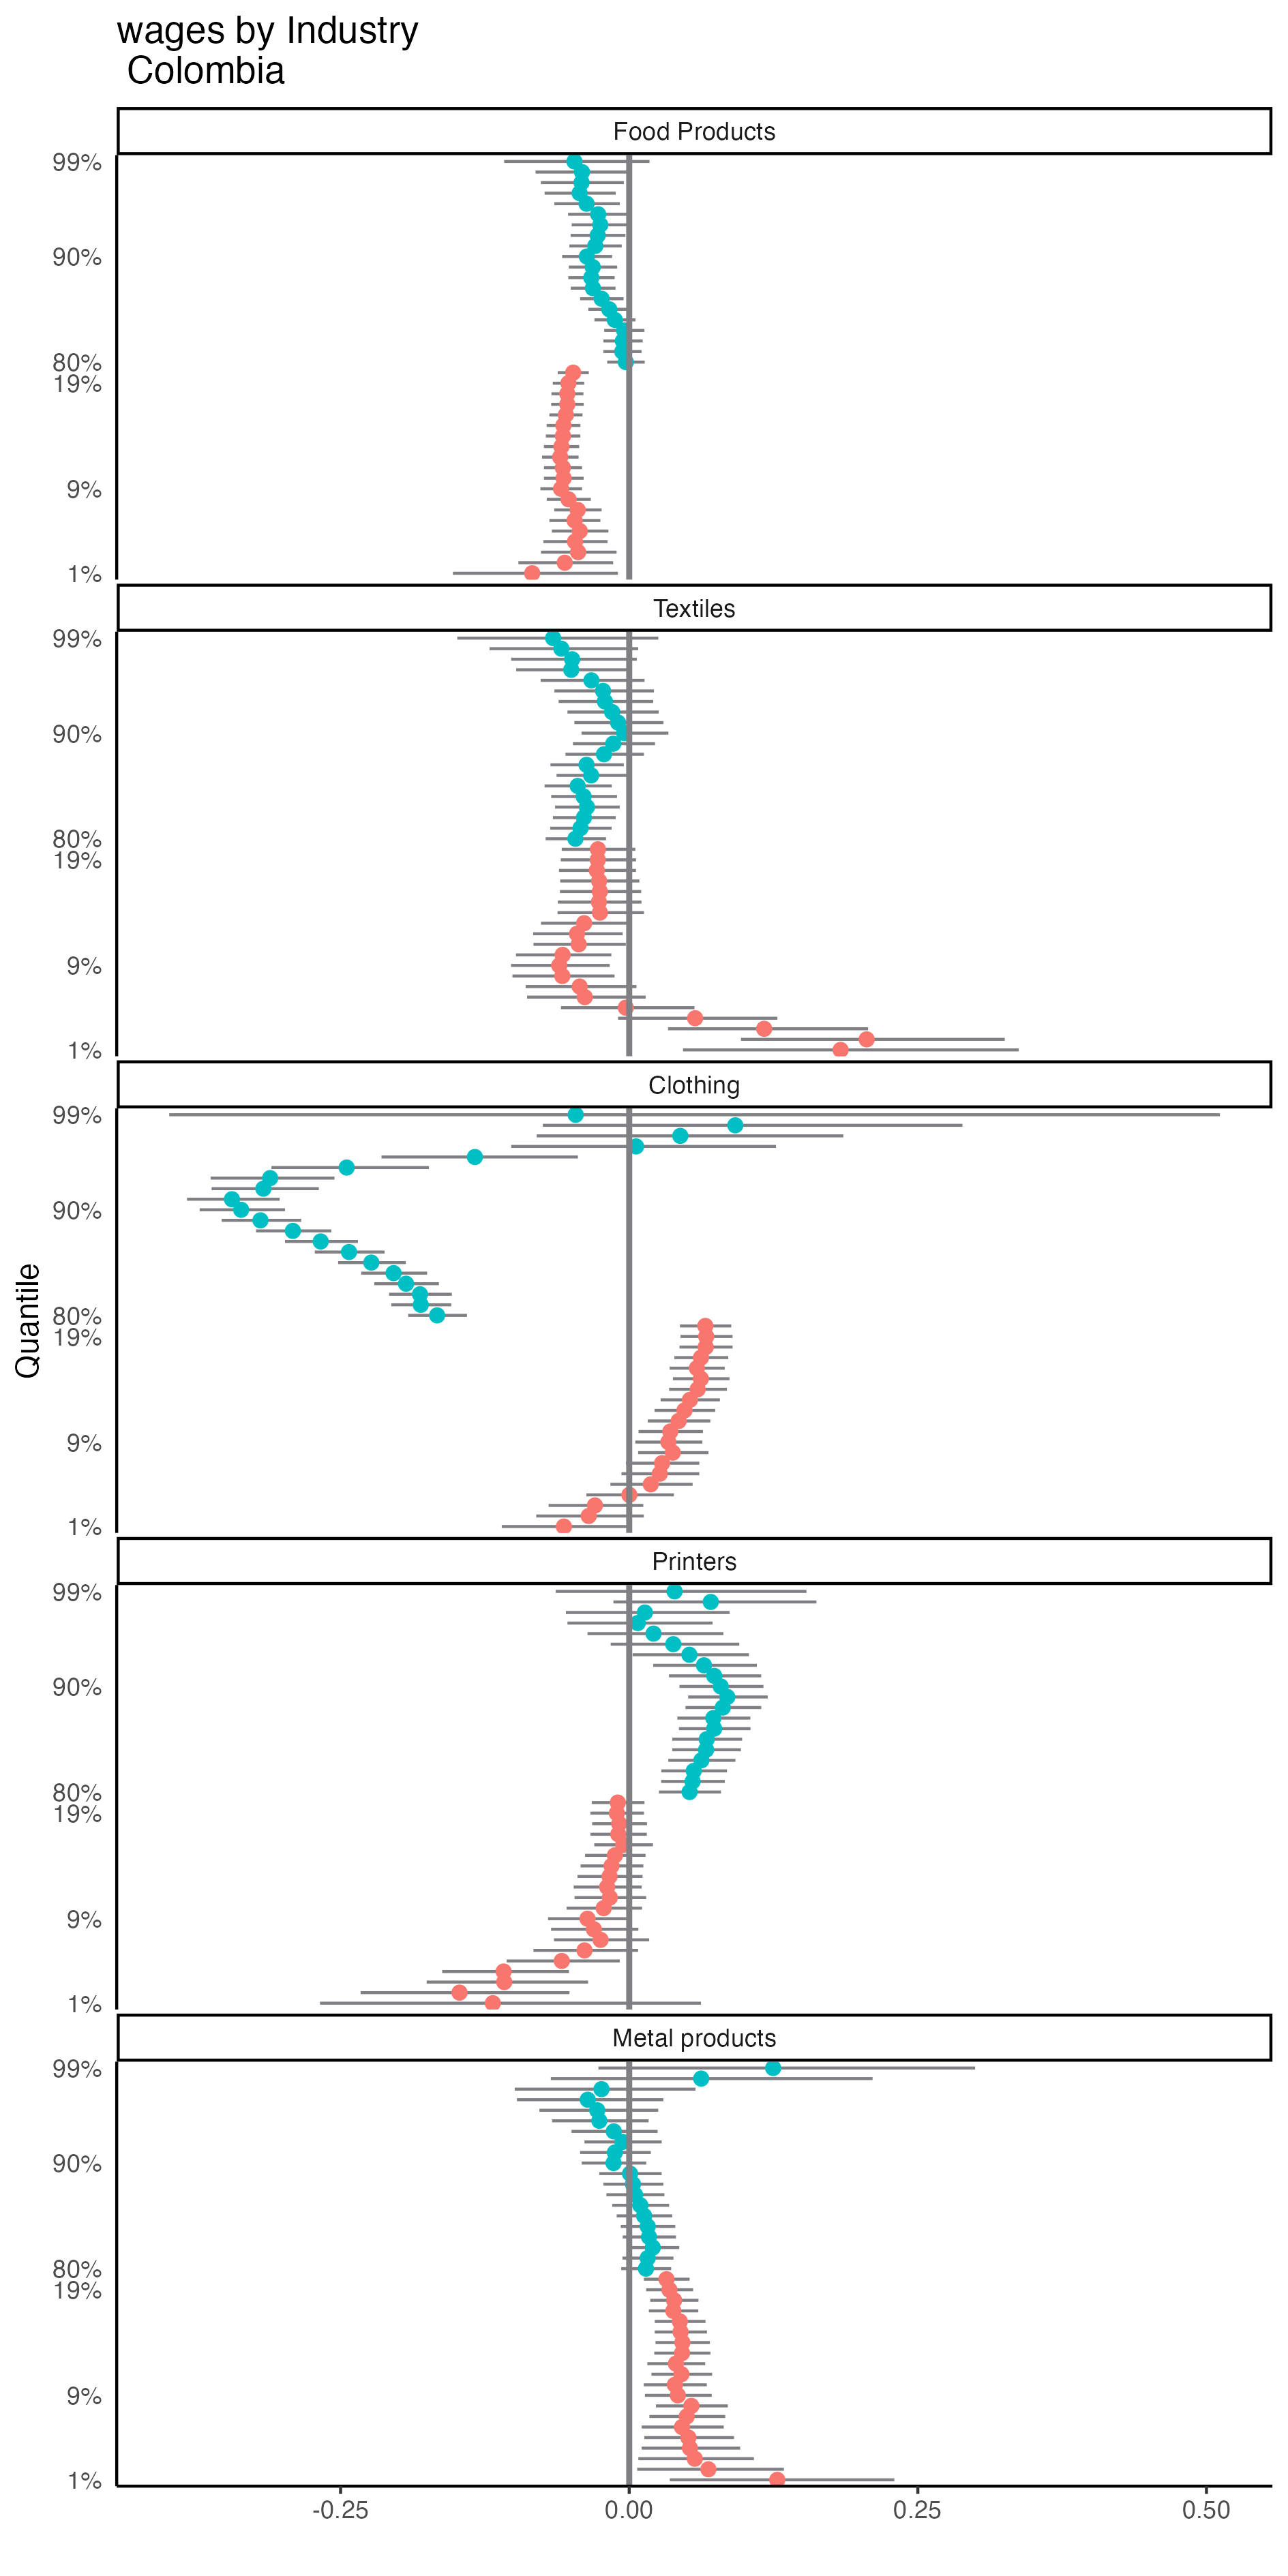
\includegraphics[width=\textwidth,height=1\textheight]{../Results/Figures/Colombia/wages_by_inds_diff.png}

}

\end{figure}


  \bibliography{biblio/export.bib,biblio/export2.bib,biblio/export31072022.bib,biblio/b100422.bib,biblio/b270123.bib}


\end{document}
